\documentclass[1p]{elsarticle_modified}
%\bibliographystyle{elsarticle-num}

%\usepackage[colorlinks]{hyperref}
%\usepackage{abbrmath_seonhwa} %\Abb, \Ascr, \Acal ,\Abf, \Afrak
\usepackage{amsfonts}
\usepackage{amssymb}
\usepackage{amsmath}
\usepackage{amsthm}
\usepackage{scalefnt}
\usepackage{amsbsy}
\usepackage{kotex}
\usepackage{caption}
\usepackage{subfig}
\usepackage{color}
\usepackage{graphicx}
\usepackage{xcolor} %% white, black, red, green, blue, cyan, magenta, yellow
\usepackage{float}
\usepackage{setspace}
\usepackage{hyperref}

\usepackage{tikz}
\usetikzlibrary{arrows}

\usepackage{multirow}
\usepackage{array} % fixed length table
\usepackage{hhline}

%%%%%%%%%%%%%%%%%%%%%
\makeatletter
\renewcommand*\env@matrix[1][\arraystretch]{%
	\edef\arraystretch{#1}%
	\hskip -\arraycolsep
	\let\@ifnextchar\new@ifnextchar
	\array{*\c@MaxMatrixCols c}}
\makeatother %https://tex.stackexchange.com/questions/14071/how-can-i-increase-the-line-spacing-in-a-matrix
%%%%%%%%%%%%%%%

\usepackage[normalem]{ulem}

\newcommand{\msout}[1]{\ifmmode\text{\sout{\ensuremath{#1}}}\else\sout{#1}\fi}
%SOURCE: \msout is \stkout macro in https://tex.stackexchange.com/questions/20609/strikeout-in-math-mode

\newcommand{\cancel}[1]{
	\ifmmode
	{\color{red}\msout{#1}}
	\else
	{\color{red}\sout{#1}}
	\fi
}

\newcommand{\add}[1]{
	{\color{blue}\uwave{#1}}
}

\newcommand{\replace}[2]{
	\ifmmode
	{\color{red}\msout{#1}}{\color{blue}\uwave{#2}}
	\else
	{\color{red}\sout{#1}}{\color{blue}\uwave{#2}}
	\fi
}

\newcommand{\Sol}{\mathcal{S}} %segment
\newcommand{\D}{D} %diagram
\newcommand{\A}{\mathcal{A}} %arc


%%%%%%%%%%%%%%%%%%%%%%%%%%%%%5 test

\def\sl{\operatorname{\textup{SL}}(2,\Cbb)}
\def\psl{\operatorname{\textup{PSL}}(2,\Cbb)}
\def\quan{\mkern 1mu \triangleright \mkern 1mu}

\theoremstyle{definition}
\newtheorem{thm}{Theorem}[section]
\newtheorem{prop}[thm]{Proposition}
\newtheorem{lem}[thm]{Lemma}
\newtheorem{ques}[thm]{Question}
\newtheorem{cor}[thm]{Corollary}
\newtheorem{defn}[thm]{Definition}
\newtheorem{exam}[thm]{Example}
\newtheorem{rmk}[thm]{Remark}
\newtheorem{alg}[thm]{Algorithm}

\newcommand{\I}{\sqrt{-1}}
\begin{document}

%\begin{frontmatter}
%
%\title{Boundary parabolic representations of knots up to 8 crossings}
%
%%% Group authors per affiliation:
%\author{Yunhi Cho} 
%\address{Department of Mathematics, University of Seoul, Seoul, Korea}
%\ead{yhcho@uos.ac.kr}
%
%
%\author{Seonhwa Kim} %\fnref{s_kim}}
%\address{Center for Geometry and Physics, Institute for Basic Science, Pohang, 37673, Korea}
%\ead{ryeona17@ibs.re.kr}
%
%\author{Hyuk Kim}
%\address{Department of Mathematical Sciences, Seoul National University, Seoul 08826, Korea}
%\ead{hyukkim@snu.ac.kr}
%
%\author{Seokbeom Yoon}
%\address{Department of Mathematical Sciences, Seoul National University, Seoul, 08826,  Korea}
%\ead{sbyoon15@snu.ac.kr}
%
%\begin{abstract}
%We find all boundary parabolic representation of knots up to 8 crossings.
%
%\end{abstract}
%\begin{keyword}
%    \MSC[2010] 57M25 
%\end{keyword}
%
%\end{frontmatter}

%\linenumbers
%\tableofcontents
%
\newcommand\colored[1]{\textcolor{white}{\rule[-0.35ex]{0.8em}{1.4ex}}\kern-0.8em\color{red} #1}%
%\newcommand\colored[1]{\textcolor{white}{ #1}\kern-2.17ex	\textcolor{white}{ #1}\kern-1.81ex	\textcolor{white}{ #1}\kern-2.15ex\color{red}#1	}

{\Large $\underline{12a_{1026}~(K12a_{1026})}$}

\setlength{\tabcolsep}{10pt}
\renewcommand{\arraystretch}{1.6}
\vspace{1cm}\begin{tabular}{m{100pt}>{\centering\arraybackslash}m{274pt}}
\multirow{5}{120pt}{
	\centering
	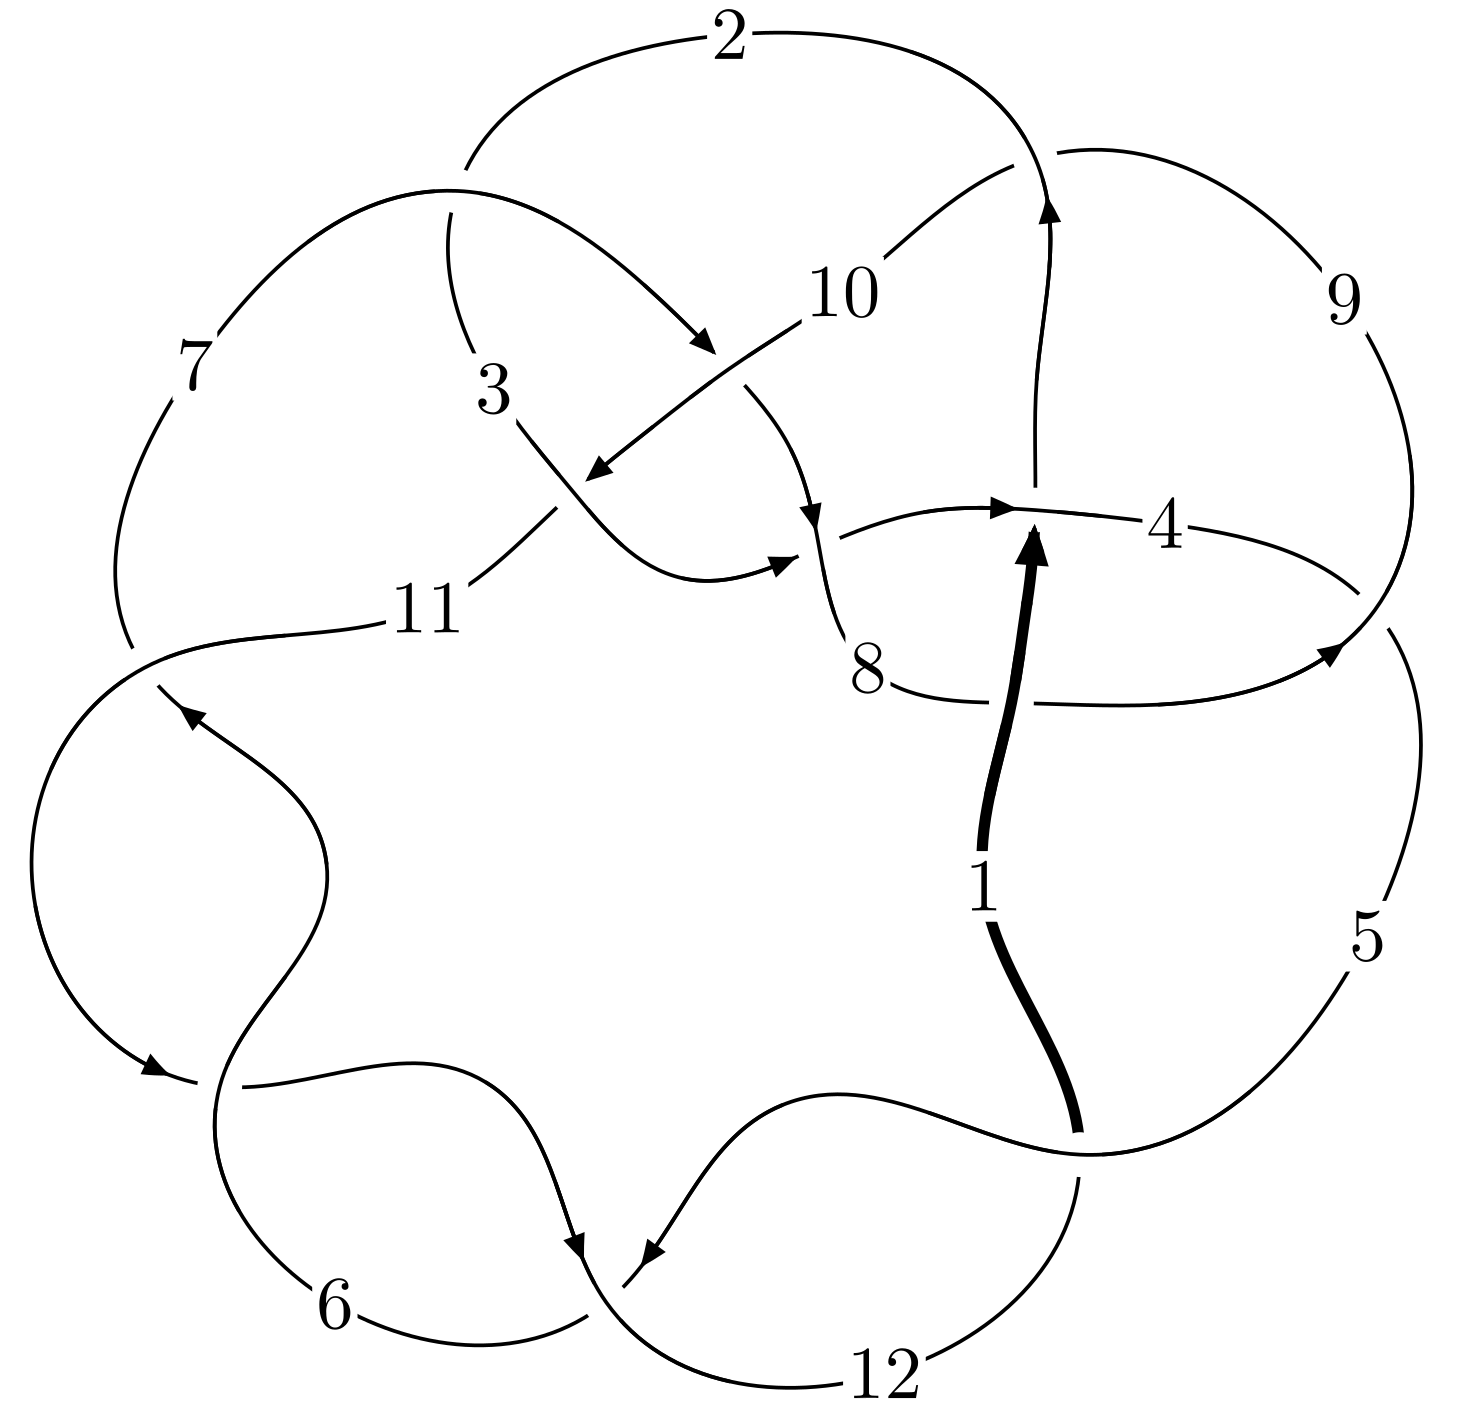
\includegraphics[width=112pt]{../../../GIT/diagram.site/Diagrams/png/1827_12a_1026.png}\\
\ \ \ A knot diagram\footnotemark}&
\allowdisplaybreaks
\textbf{Linearized knot diagam} \\
\cline{2-2}
 &
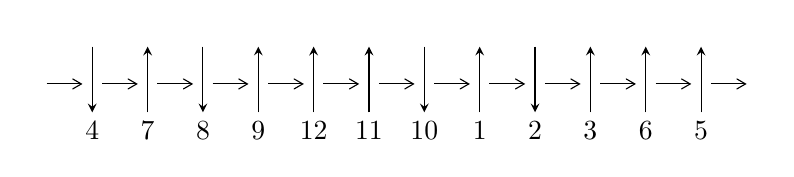
\begin{tikzpicture}[x=20pt, y=17pt]
	% nodes
	\node (C0) at (0, 0) {};
	\node (C1) at (1, 0) {};
	\node (C1U) at (1, +1) {};
	\node (C1D) at (1, -1) {4};

	\node (C2) at (2, 0) {};
	\node (C2U) at (2, +1) {};
	\node (C2D) at (2, -1) {7};

	\node (C3) at (3, 0) {};
	\node (C3U) at (3, +1) {};
	\node (C3D) at (3, -1) {8};

	\node (C4) at (4, 0) {};
	\node (C4U) at (4, +1) {};
	\node (C4D) at (4, -1) {9};

	\node (C5) at (5, 0) {};
	\node (C5U) at (5, +1) {};
	\node (C5D) at (5, -1) {12};

	\node (C6) at (6, 0) {};
	\node (C6U) at (6, +1) {};
	\node (C6D) at (6, -1) {11};

	\node (C7) at (7, 0) {};
	\node (C7U) at (7, +1) {};
	\node (C7D) at (7, -1) {10};

	\node (C8) at (8, 0) {};
	\node (C8U) at (8, +1) {};
	\node (C8D) at (8, -1) {1};

	\node (C9) at (9, 0) {};
	\node (C9U) at (9, +1) {};
	\node (C9D) at (9, -1) {2};

	\node (C10) at (10, 0) {};
	\node (C10U) at (10, +1) {};
	\node (C10D) at (10, -1) {3};

	\node (C11) at (11, 0) {};
	\node (C11U) at (11, +1) {};
	\node (C11D) at (11, -1) {6};

	\node (C12) at (12, 0) {};
	\node (C12U) at (12, +1) {};
	\node (C12D) at (12, -1) {5};
	\node (C13) at (13, 0) {};

	% arrows
	\draw[->,>={angle 60}]
	(C0) edge (C1) (C1) edge (C2) (C2) edge (C3) (C3) edge (C4) (C4) edge (C5) (C5) edge (C6) (C6) edge (C7) (C7) edge (C8) (C8) edge (C9) (C9) edge (C10) (C10) edge (C11) (C11) edge (C12) (C12) edge (C13) ;	\draw[->,>=stealth]
	(C1U) edge (C1D) (C2D) edge (C2U) (C3U) edge (C3D) (C4D) edge (C4U) (C5D) edge (C5U) (C6D) edge (C6U) (C7U) edge (C7D) (C8D) edge (C8U) (C9U) edge (C9D) (C10D) edge (C10U) (C11D) edge (C11U) (C12D) edge (C12U) ;
	\end{tikzpicture} \\
\hhline{~~} \\& 
\textbf{Solving Sequence} \\ \cline{2-2} 
 &
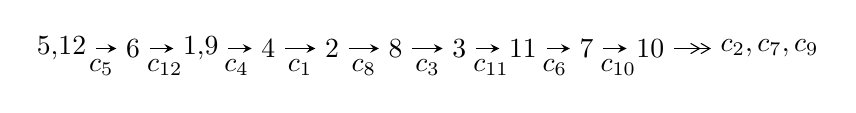
\begin{tikzpicture}[x=23pt, y=7pt]
	% node
	\node (A0) at (-1/8, 0) {5,12};
	\node (A1) at (1, 0) {6};
	\node (A2) at (33/16, 0) {1,9};
	\node (A3) at (25/8, 0) {4};
	\node (A4) at (33/8, 0) {2};
	\node (A5) at (41/8, 0) {8};
	\node (A6) at (49/8, 0) {3};
	\node (A7) at (57/8, 0) {11};
	\node (A8) at (65/8, 0) {7};
	\node (A9) at (73/8, 0) {10};
	\node (C1) at (1/2, -1) {$c_{5}$};
	\node (C2) at (3/2, -1) {$c_{12}$};
	\node (C3) at (21/8, -1) {$c_{4}$};
	\node (C4) at (29/8, -1) {$c_{1}$};
	\node (C5) at (37/8, -1) {$c_{8}$};
	\node (C6) at (45/8, -1) {$c_{3}$};
	\node (C7) at (53/8, -1) {$c_{11}$};
	\node (C8) at (61/8, -1) {$c_{6}$};
	\node (C9) at (69/8, -1) {$c_{10}$};
	\node (A10) at (11, 0) {$c_{2},c_{7},c_{9}$};

	% edge
	\draw[->,>=stealth]	
	(A0) edge (A1) (A1) edge (A2) (A2) edge (A3) (A3) edge (A4) (A4) edge (A5) (A5) edge (A6) (A6) edge (A7) (A7) edge (A8) (A8) edge (A9) ;
	\draw[->>,>={angle 60}]	
	(A9) edge (A10);
\end{tikzpicture} \\ 

\end{tabular} \\

\footnotetext{
The image of knot diagram is generated by the software ``\textbf{Draw programme}" developed by Andrew Bartholomew(\url{http://www.layer8.co.uk/maths/draw/index.htm\#Running-draw}), where we modified some parts for our purpose(\url{https://github.com/CATsTAILs/LinksPainter}).
}\phantom \\ \newline 
\centering \textbf{Ideals for irreducible components\footnotemark of $X_{\text{par}}$} 
 
\begin{align*}
I^u_{1}&=\langle 
-3 u^{12}+17 u^{11}+\cdots+10 b-42,\;9 u^{12}-46 u^{11}+\cdots+40 a+196,\;u^{13}-6 u^{12}+\cdots+52 u-8\rangle \\
I^u_{2}&=\langle 
u^7 a-2 u^6 a+8 u^5 a-10 u^4 a+19 u^3 a-12 u^2 a+15 a u+5 b-4 a,\;4 u^6 a+u^7+\cdots+20 a-6,\\
\phantom{I^u_{2}}&\phantom{= \langle  }u^8-3 u^7+10 u^6-18 u^5+29 u^4-31 u^3+27 u^2-14 u+4\rangle \\
I^u_{3}&=\langle 
13 u^4 a^3-3 u^4 a^2+\cdots+69 a-1,\;-2 u^4 a^3- u^4 a+\cdots+6 a+2,\;u^5+u^4+4 u^3+3 u^2+3 u+1\rangle \\
I^u_{4}&=\langle 
-1.98276\times10^{25} a^{7} u^{4}+9.89103\times10^{25} a^{6} u^{4}+\cdots-5.40442\times10^{26} a+1.69204\times10^{27},\\
\phantom{I^u_{4}}&\phantom{= \langle  }2 a^7 u^4+3 a^6 u^4+\cdots+299 a+412,\;u^5+u^4+4 u^3+3 u^2+3 u+1\rangle \\
I^u_{5}&=\langle 
u^{19}+u^{18}+\cdots+2 b+7,\;6 u^{19}+26 u^{18}+\cdots+26 a+299,\\
\phantom{I^u_{5}}&\phantom{= \langle  }u^{20}+14 u^{18}+83 u^{16}+274 u^{14}+562 u^{12}+767 u^{10}+738 u^8+519 u^6+261 u^4+85 u^2+13\rangle \\
I^u_{6}&=\langle 
- u^4+u^3-3 u^2+b+2 u-1,\;u^3+a+2 u,\;u^5- u^4+4 u^3-3 u^2+3 u-1\rangle \\
I^u_{7}&=\langle 
u^4 a+2 u^4+4 u^2 a+3 u^3- a u+8 u^2+3 b+a+7 u+5,\\
\phantom{I^u_{7}}&\phantom{= \langle  }2 u^4 a+u^3 a+6 u^2 a- u^3+a^2+2 a u- u^2+2 a-3 u+1,\;u^5+u^4+4 u^3+3 u^2+3 u+1\rangle \\
I^u_{8}&=\langle 
2 b- u+1,\;3 a-2 u,\;u^2+3\rangle \\
I^u_{9}&=\langle 
b^2- b+1,\;a,\;u-1\rangle \\
\\
I^v_{1}&=\langle 
a,\;b^2+b+1,\;v+1\rangle \\
\end{align*}
\raggedright * 10 irreducible components of $\dim_{\mathbb{C}}=0$, with total 130 representations.\\
\footnotetext{All coefficients of polynomials are rational numbers. But the coefficients are sometimes approximated in decimal forms when there is not enough margin.}
\newpage
\renewcommand{\arraystretch}{1}
\centering \section*{I. $I^u_{1}= \langle -3 u^{12}+17 u^{11}+\cdots+10 b-42,\;9 u^{12}-46 u^{11}+\cdots+40 a+196,\;u^{13}-6 u^{12}+\cdots+52 u-8 \rangle$}
\flushleft \textbf{(i) Arc colorings}\\
\begin{tabular}{m{7pt} m{180pt} m{7pt} m{180pt} }
\flushright $a_{5}=$&$\begin{pmatrix}1\\0\end{pmatrix}$ \\
\flushright $a_{12}=$&$\begin{pmatrix}0\\u\end{pmatrix}$ \\
\flushright $a_{6}=$&$\begin{pmatrix}1\\- u^2\end{pmatrix}$ \\
\flushright $a_{1}=$&$\begin{pmatrix}u\\u\end{pmatrix}$ \\
\flushright $a_{9}=$&$\begin{pmatrix}-0.225000 u^{12}+1.15000 u^{11}+\cdots+20.4000 u-4.90000\\\frac{3}{10} u^{12}-\frac{17}{10} u^{11}+\cdots-\frac{91}{5} u+\frac{21}{5}\end{pmatrix}$ \\
\flushright $a_{4}=$&$\begin{pmatrix}-0.175000 u^{12}+0.700000 u^{11}+\cdots-0.300000 u+0.300000\\0.650000 u^{12}-3.60000 u^{11}+\cdots-35.6000 u+6.60000\end{pmatrix}$ \\
\flushright $a_{2}=$&$\begin{pmatrix}0.325000 u^{12}-1.55000 u^{11}+\cdots-10.8000 u+2.30000\\-\frac{2}{5} u^{12}+\frac{21}{10} u^{11}+\cdots+\frac{43}{5} u-\frac{3}{5}\end{pmatrix}$ \\
\flushright $a_{8}=$&$\begin{pmatrix}-0.325000 u^{12}+2.05000 u^{11}+\cdots+31.8000 u-7.30000\\\frac{1}{5} u^{12}-\frac{4}{5} u^{11}+\cdots-\frac{34}{5} u+\frac{9}{5}\end{pmatrix}$ \\
\flushright $a_{3}=$&$\begin{pmatrix}0.325000 u^{12}-2.05000 u^{11}+\cdots-31.8000 u+7.30000\\\frac{2}{5} u^{12}-\frac{21}{10} u^{11}+\cdots-\frac{73}{5} u+\frac{13}{5}\end{pmatrix}$ \\
\flushright $a_{11}=$&$\begin{pmatrix}- u\\u^3+u\end{pmatrix}$ \\
\flushright $a_{7}=$&$\begin{pmatrix}u^2+1\\- u^4-2 u^2\end{pmatrix}$ \\
\flushright $a_{10}=$&$\begin{pmatrix}-0.475000 u^{12}+2.40000 u^{11}+\cdots+25.9000 u-5.90000\\\frac{1}{20} u^{12}-\frac{1}{5} u^{11}+\cdots-\frac{51}{5} u+\frac{11}{5}\end{pmatrix}$\\&\end{tabular}
\flushleft \textbf{(ii) Obstruction class $= -1$}\\~\\
\flushleft \textbf{(iii) Cusp Shapes $= \frac{7}{10} u^{12}-\frac{24}{5} u^{11}+\frac{199}{10} u^{10}-62 u^9+\frac{722}{5} u^8-\frac{1386}{5} u^7+\frac{2109}{5} u^6-\frac{2659}{5} u^5+\frac{5333}{10} u^4-\frac{2156}{5} u^3+\frac{1341}{5} u^2-\frac{644}{5} u+\frac{194}{5}$}\\~\\
\newpage\renewcommand{\arraystretch}{1}
\flushleft \textbf{(iv) u-Polynomials at the component}\newline \\
\begin{tabular}{m{50pt}|m{274pt}}
Crossings & \hspace{64pt}u-Polynomials at each crossing \\
\hline $$\begin{aligned}c_{1},c_{7}\end{aligned}$$&$\begin{aligned}
&u^{13}-11 u^{12}+\cdots+107 u+7
\end{aligned}$\\
\hline $$\begin{aligned}c_{2},c_{4},c_{8}\\c_{10}\end{aligned}$$&$\begin{aligned}
&u^{13}+u^{12}+3 u^{11}+u^{10}+9 u^9+5 u^8+9 u^7+u^6+6 u^5-2 u^3- u-1
\end{aligned}$\\
\hline $$\begin{aligned}c_{3},c_{9}\end{aligned}$$&$\begin{aligned}
&u^{13}-2 u^{12}+\cdots+7 u-24
\end{aligned}$\\
\hline $$\begin{aligned}c_{5},c_{6},c_{11}\\c_{12}\end{aligned}$$&$\begin{aligned}
&u^{13}-6 u^{12}+\cdots+52 u-8
\end{aligned}$\\
\hline
\end{tabular}\\~\\
\newpage\renewcommand{\arraystretch}{1}
\flushleft \textbf{(v) Riley Polynomials at the component}\newline \\
\begin{tabular}{m{50pt}|m{274pt}}
Crossings & \hspace{64pt}Riley Polynomials at each crossing \\
\hline $$\begin{aligned}c_{1},c_{7}\end{aligned}$$&$\begin{aligned}
&y^{13}+3 y^{12}+\cdots+15999 y-49
\end{aligned}$\\
\hline $$\begin{aligned}c_{2},c_{4},c_{8}\\c_{10}\end{aligned}$$&$\begin{aligned}
&y^{13}+5 y^{12}+\cdots+y-1
\end{aligned}$\\
\hline $$\begin{aligned}c_{3},c_{9}\end{aligned}$$&$\begin{aligned}
&y^{13}-18 y^{12}+\cdots+4849 y-576
\end{aligned}$\\
\hline $$\begin{aligned}c_{5},c_{6},c_{11}\\c_{12}\end{aligned}$$&$\begin{aligned}
&y^{13}+14 y^{12}+\cdots+208 y-64
\end{aligned}$\\
\hline
\end{tabular}\\~\\
\newpage\flushleft \textbf{(vi) Complex Volumes and Cusp Shapes}
$$\begin{array}{c|c|c}  
\text{Solutions to }I^u_{1}& \I (\text{vol} + \sqrt{-1}CS) & \text{Cusp shape}\\
 \hline 
\begin{aligned}
u &= \phantom{-}0.925588 + 0.229213 I \\
a &= \phantom{-}0.251266 - 0.164394 I \\
b &= -0.719509 - 0.945453 I\end{aligned}
 & -2.64658 + 9.80964 I & \phantom{-}0.48730 - 9.61538 I \\ \hline\begin{aligned}
u &= \phantom{-}0.925588 - 0.229213 I \\
a &= \phantom{-}0.251266 + 0.164394 I \\
b &= -0.719509 + 0.945453 I\end{aligned}
 & -2.64658 - 9.80964 I & \phantom{-}0.48730 + 9.61538 I \\ \hline\begin{aligned}
u &= -0.012360 + 0.896275 I \\
a &= -0.353446 - 0.826500 I \\
b &= -0.562920 - 0.195545 I\end{aligned}
 & -1.71733 + 1.71633 I & \phantom{-}2.68735 - 4.73670 I \\ \hline\begin{aligned}
u &= -0.012360 - 0.896275 I \\
a &= -0.353446 + 0.826500 I \\
b &= -0.562920 + 0.195545 I\end{aligned}
 & -1.71733 - 1.71633 I & \phantom{-}2.68735 + 4.73670 I \\ \hline\begin{aligned}
u &= \phantom{-}0.548935 + 1.070790 I \\
a &= -0.33469 + 1.40815 I \\
b &= \phantom{-}0.89400 + 1.20313 I\end{aligned}
 & -6.6253 + 14.6812 I & -1.43670 - 9.72736 I \\ \hline\begin{aligned}
u &= \phantom{-}0.548935 - 1.070790 I \\
a &= -0.33469 - 1.40815 I \\
b &= \phantom{-}0.89400 - 1.20313 I\end{aligned}
 & -6.6253 - 14.6812 I & -1.43670 + 9.72736 I \\ \hline\begin{aligned}
u &= \phantom{-}0.959730 + 0.890724 I \\
a &= \phantom{-}0.549017 - 0.142828 I \\
b &= \phantom{-}0.361184 - 0.750707 I\end{aligned}
 & -4.30776 - 3.71769 I & -7.51801 + 8.71663 I \\ \hline\begin{aligned}
u &= \phantom{-}0.959730 - 0.890724 I \\
a &= \phantom{-}0.549017 + 0.142828 I \\
b &= \phantom{-}0.361184 + 0.750707 I\end{aligned}
 & -4.30776 + 3.71769 I & -7.51801 - 8.71663 I \\ \hline\begin{aligned}
u &= \phantom{-}0.418088\phantom{ +0.000000I} \\
a &= -0.957441\phantom{ +0.000000I} \\
b &= \phantom{-}0.687897\phantom{ +0.000000I}\end{aligned}
 & \phantom{-}0.881810\phantom{ +0.000000I} & \phantom{-}11.5670\phantom{ +0.000000I} \\ \hline\begin{aligned}
u &= \phantom{-}0.15342 + 1.73647 I \\
a &= -0.13933 - 1.90579 I \\
b &= -0.99446 - 1.40865 I\end{aligned}
 & -16.4057 + 17.5804 I & -2.58727 - 8.30259 I\\
 \hline 
 \end{array}$$\newpage$$\begin{array}{c|c|c}  
\text{Solutions to }I^u_{1}& \I (\text{vol} + \sqrt{-1}CS) & \text{Cusp shape}\\
 \hline 
\begin{aligned}
u &= \phantom{-}0.15342 - 1.73647 I \\
a &= -0.13933 + 1.90579 I \\
b &= -0.99446 + 1.40865 I\end{aligned}
 & -16.4057 - 17.5804 I & -2.58727 + 8.30259 I \\ \hline\begin{aligned}
u &= \phantom{-}0.21564 + 1.85083 I \\
a &= -0.244097 + 0.817556 I \\
b &= \phantom{-}0.177755 + 0.770665 I\end{aligned}
 & -13.97390 + 1.53205 I & -8.41618 - 4.24758 I \\ \hline\begin{aligned}
u &= \phantom{-}0.21564 - 1.85083 I \\
a &= -0.244097 - 0.817556 I \\
b &= \phantom{-}0.177755 - 0.770665 I\end{aligned}
 & -13.97390 - 1.53205 I & -8.41618 + 4.24758 I\\
 \hline 
 \end{array}$$\newpage\newpage\renewcommand{\arraystretch}{1}
\centering \section*{II. $I^u_{2}= \langle u^7 a-2 u^6 a+\cdots+5 b-4 a,\;4 u^6 a+u^7+\cdots+20 a-6,\;u^8-3 u^7+\cdots-14 u+4 \rangle$}
\flushleft \textbf{(i) Arc colorings}\\
\begin{tabular}{m{7pt} m{180pt} m{7pt} m{180pt} }
\flushright $a_{5}=$&$\begin{pmatrix}1\\0\end{pmatrix}$ \\
\flushright $a_{12}=$&$\begin{pmatrix}0\\u\end{pmatrix}$ \\
\flushright $a_{6}=$&$\begin{pmatrix}1\\- u^2\end{pmatrix}$ \\
\flushright $a_{1}=$&$\begin{pmatrix}u\\u\end{pmatrix}$ \\
\flushright $a_{9}=$&$\begin{pmatrix}a\\-\frac{1}{5} u^7 a+\frac{2}{5} u^6 a+\cdots-3 a u+\frac{4}{5} a\end{pmatrix}$ \\
\flushright $a_{4}=$&$\begin{pmatrix}\frac{1}{2} u^7 a-\frac{3}{2} u^6 a+\cdots-2 a+\frac{1}{2}\\-\frac{1}{5} u^7 a-\frac{1}{2} u^7+\cdots+\frac{14}{5} a+2\end{pmatrix}$ \\
\flushright $a_{2}=$&$\begin{pmatrix}-\frac{1}{5} u^7 a-\frac{1}{2} u^7+\cdots+\frac{9}{5} a+\frac{5}{2}\\\frac{2}{5} u^7 a+\frac{1}{2} u^7+\cdots-\frac{8}{5} a-2\end{pmatrix}$ \\
\flushright $a_{8}=$&$\begin{pmatrix}\frac{1}{5} u^7 a-\frac{2}{5} u^6 a+\cdots+2 a u+\frac{1}{5} a\\- a u\end{pmatrix}$ \\
\flushright $a_{3}=$&$\begin{pmatrix}\frac{1}{5} u^7 a-\frac{2}{5} u^6 a+\cdots+\frac{1}{5} a+\frac{1}{2}\\-\frac{1}{5} u^7 a-\frac{1}{2} u^7+\cdots+\frac{4}{5} a+2\end{pmatrix}$ \\
\flushright $a_{11}=$&$\begin{pmatrix}- u\\u^3+u\end{pmatrix}$ \\
\flushright $a_{7}=$&$\begin{pmatrix}u^2+1\\- u^4-2 u^2\end{pmatrix}$ \\
\flushright $a_{10}=$&$\begin{pmatrix}-\frac{7}{10} u^7 a-\frac{1}{4} u^7+\cdots+\frac{14}{5} a+\frac{3}{2}\\-\frac{4}{5} u^7 a+\frac{8}{5} u^6 a+\cdots+\frac{6}{5} a+1\end{pmatrix}$\\&\end{tabular}
\flushleft \textbf{(ii) Obstruction class $= -1$}\\~\\
\flushleft \textbf{(iii) Cusp Shapes $= -4 u^7+15 u^6-41 u^5+79 u^4-104 u^3+107 u^2-70 u+30$}\\~\\
\newpage\renewcommand{\arraystretch}{1}
\flushleft \textbf{(iv) u-Polynomials at the component}\newline \\
\begin{tabular}{m{50pt}|m{274pt}}
Crossings & \hspace{64pt}u-Polynomials at each crossing \\
\hline $$\begin{aligned}c_{1},c_{7}\end{aligned}$$&$\begin{aligned}
&u^{16}-13 u^{15}+\cdots-328 u+41
\end{aligned}$\\
\hline $$\begin{aligned}c_{2},c_{4},c_{8}\\c_{10}\end{aligned}$$&$\begin{aligned}
&u^{16}+u^{15}+\cdots-2 u+1
\end{aligned}$\\
\hline $$\begin{aligned}c_{3},c_{9}\end{aligned}$$&$\begin{aligned}
&(u^8- u^6- u^3+2 u^2- u+1)^2
\end{aligned}$\\
\hline $$\begin{aligned}c_{5},c_{6},c_{11}\\c_{12}\end{aligned}$$&$\begin{aligned}
&(u^8-3 u^7+10 u^6-18 u^5+29 u^4-31 u^3+27 u^2-14 u+4)^2
\end{aligned}$\\
\hline
\end{tabular}\\~\\
\newpage\renewcommand{\arraystretch}{1}
\flushleft \textbf{(v) Riley Polynomials at the component}\newline \\
\begin{tabular}{m{50pt}|m{274pt}}
Crossings & \hspace{64pt}Riley Polynomials at each crossing \\
\hline $$\begin{aligned}c_{1},c_{7}\end{aligned}$$&$\begin{aligned}
&y^{16}+y^{15}+\cdots+2788 y+1681
\end{aligned}$\\
\hline $$\begin{aligned}c_{2},c_{4},c_{8}\\c_{10}\end{aligned}$$&$\begin{aligned}
&y^{16}+7 y^{15}+\cdots-6 y+1
\end{aligned}$\\
\hline $$\begin{aligned}c_{3},c_{9}\end{aligned}$$&$\begin{aligned}
&(y^8-2 y^7+y^6+4 y^5-2 y^4-3 y^3+2 y^2+3 y+1)^2
\end{aligned}$\\
\hline $$\begin{aligned}c_{5},c_{6},c_{11}\\c_{12}\end{aligned}$$&$\begin{aligned}
&(y^8+11 y^7+50 y^6+124 y^5+189 y^4+181 y^3+93 y^2+20 y+16)^2
\end{aligned}$\\
\hline
\end{tabular}\\~\\
\newpage\flushleft \textbf{(vi) Complex Volumes and Cusp Shapes}
$$\begin{array}{c|c|c}  
\text{Solutions to }I^u_{2}& \I (\text{vol} + \sqrt{-1}CS) & \text{Cusp shape}\\
 \hline 
\begin{aligned}
u &= \phantom{-}0.673128 + 1.045810 I \\
a &= \phantom{-}0.301794 - 1.174260 I \\
b &= -0.803268 - 1.117440 I\end{aligned}
 & -6.47283 + 5.59386 I & -6.60310 - 4.62010 I \\ \hline\begin{aligned}
u &= \phantom{-}0.673128 + 1.045810 I \\
a &= -0.633138 + 0.444550 I \\
b &= -0.073509 + 0.875041 I\end{aligned}
 & -6.47283 + 5.59386 I & -6.60310 - 4.62010 I \\ \hline\begin{aligned}
u &= \phantom{-}0.673128 - 1.045810 I \\
a &= \phantom{-}0.301794 + 1.174260 I \\
b &= -0.803268 + 1.117440 I\end{aligned}
 & -6.47283 - 5.59386 I & -6.60310 + 4.62010 I \\ \hline\begin{aligned}
u &= \phantom{-}0.673128 - 1.045810 I \\
a &= -0.633138 - 0.444550 I \\
b &= -0.073509 - 0.875041 I\end{aligned}
 & -6.47283 - 5.59386 I & -6.60310 + 4.62010 I \\ \hline\begin{aligned}
u &= \phantom{-}0.504550 + 0.414188 I \\
a &= -0.841060 + 0.591436 I \\
b &= \phantom{-}0.745591 + 0.724115 I\end{aligned}
 & \phantom{-}1.86670 + 1.71603 I & \phantom{-}7.94168 - 3.64767 I \\ \hline\begin{aligned}
u &= \phantom{-}0.504550 + 0.414188 I \\
a &= -0.275916 - 0.687804 I \\
b &= -0.631239 + 0.403393 I\end{aligned}
 & \phantom{-}1.86670 + 1.71603 I & \phantom{-}7.94168 - 3.64767 I \\ \hline\begin{aligned}
u &= \phantom{-}0.504550 - 0.414188 I \\
a &= -0.841060 - 0.591436 I \\
b &= \phantom{-}0.745591 - 0.724115 I\end{aligned}
 & \phantom{-}1.86670 - 1.71603 I & \phantom{-}7.94168 + 3.64767 I \\ \hline\begin{aligned}
u &= \phantom{-}0.504550 - 0.414188 I \\
a &= -0.275916 + 0.687804 I \\
b &= -0.631239 - 0.403393 I\end{aligned}
 & \phantom{-}1.86670 - 1.71603 I & \phantom{-}7.94168 + 3.64767 I \\ \hline\begin{aligned}
u &= \phantom{-}0.143098 + 1.398100 I \\
a &= \phantom{-}0.462450 + 0.187513 I \\
b &= \phantom{-}0.412575 - 0.112689 I\end{aligned}
 & -3.91396 + 3.96633 I & \phantom{-}6.91340 + 0.89673 I \\ \hline\begin{aligned}
u &= \phantom{-}0.143098 + 1.398100 I \\
a &= \phantom{-}0.01496 - 1.62294 I \\
b &= -0.833636 - 1.113530 I\end{aligned}
 & -3.91396 + 3.96633 I & \phantom{-}6.91340 + 0.89673 I\\
 \hline 
 \end{array}$$\newpage$$\begin{array}{c|c|c}  
\text{Solutions to }I^u_{2}& \I (\text{vol} + \sqrt{-1}CS) & \text{Cusp shape}\\
 \hline 
\begin{aligned}
u &= \phantom{-}0.143098 - 1.398100 I \\
a &= \phantom{-}0.462450 - 0.187513 I \\
b &= \phantom{-}0.412575 + 0.112689 I\end{aligned}
 & -3.91396 - 3.96633 I & \phantom{-}6.91340 - 0.89673 I \\ \hline\begin{aligned}
u &= \phantom{-}0.143098 - 1.398100 I \\
a &= \phantom{-}0.01496 + 1.62294 I \\
b &= -0.833636 + 1.113530 I\end{aligned}
 & -3.91396 - 3.96633 I & \phantom{-}6.91340 - 0.89673 I \\ \hline\begin{aligned}
u &= \phantom{-}0.17922 + 1.74365 I \\
a &= \phantom{-}0.360792 - 1.135170 I \\
b &= -0.251883 - 1.053690 I\end{aligned}
 & -16.1539 + 9.0459 I & -5.25198 - 5.62090 I \\ \hline\begin{aligned}
u &= \phantom{-}0.17922 + 1.74365 I \\
a &= \phantom{-}0.11012 + 1.80963 I \\
b &= \phantom{-}0.93537 + 1.35801 I\end{aligned}
 & -16.1539 + 9.0459 I & -5.25198 - 5.62090 I \\ \hline\begin{aligned}
u &= \phantom{-}0.17922 - 1.74365 I \\
a &= \phantom{-}0.360792 + 1.135170 I \\
b &= -0.251883 + 1.053690 I\end{aligned}
 & -16.1539 - 9.0459 I & -5.25198 + 5.62090 I \\ \hline\begin{aligned}
u &= \phantom{-}0.17922 - 1.74365 I \\
a &= \phantom{-}0.11012 - 1.80963 I \\
b &= \phantom{-}0.93537 - 1.35801 I\end{aligned}
 & -16.1539 - 9.0459 I & -5.25198 + 5.62090 I\\
 \hline 
 \end{array}$$\newpage\newpage\renewcommand{\arraystretch}{1}
\centering \section*{III. $I^u_{3}= \langle 13 u^4 a^3-3 u^4 a^2+\cdots+69 a-1,\;-2 u^4 a^3- u^4 a+\cdots+6 a+2,\;u^5+u^4+4 u^3+3 u^2+3 u+1 \rangle$}
\flushleft \textbf{(i) Arc colorings}\\
\begin{tabular}{m{7pt} m{180pt} m{7pt} m{180pt} }
\flushright $a_{5}=$&$\begin{pmatrix}1\\0\end{pmatrix}$ \\
\flushright $a_{12}=$&$\begin{pmatrix}0\\u\end{pmatrix}$ \\
\flushright $a_{6}=$&$\begin{pmatrix}1\\- u^2\end{pmatrix}$ \\
\flushright $a_{1}=$&$\begin{pmatrix}u\\u\end{pmatrix}$ \\
\flushright $a_{9}=$&$\begin{pmatrix}a\\-1.44444 a^{3} u^{4}+0.333333 a^{2} u^{4}+\cdots-7.66667 a+0.111111\end{pmatrix}$ \\
\flushright $a_{4}=$&$\begin{pmatrix}\frac{2}{9} u^4 a^3+\frac{2}{3} u^4 a^2+\cdots-\frac{1}{3} a-\frac{2}{9}\\-2.44444 a^{3} u^{4}+2.66667 a^{2} u^{4}+\cdots-17.3333 a-5.55556\end{pmatrix}$ \\
\flushright $a_{2}=$&$\begin{pmatrix}\frac{13}{9} u^4 a^3-\frac{1}{3} u^4 a^2+\cdots+\frac{20}{3} a-\frac{1}{9}\\-1.22222 a^{3} u^{4}+1.66667 a^{2} u^{4}+\cdots-10.3333 a-2.44444\end{pmatrix}$ \\
\flushright $a_{8}=$&$\begin{pmatrix}-0.222222 a^{3} u^{4}-1.33333 a^{2} u^{4}+\cdots+3.66667 a+2.55556\\-\frac{5}{3} u^4 a^3- u^4 a^2+\cdots-5 a+\frac{8}{3}\end{pmatrix}$ \\
\flushright $a_{3}=$&$\begin{pmatrix}\frac{2}{9} u^4 a^3+\frac{4}{3} u^4 a^2+\cdots-\frac{11}{3} a-\frac{23}{9}\\-1.55556 a^{3} u^{4}-0.333333 a^{2} u^{4}+\cdots-5.33333 a+0.888889\end{pmatrix}$ \\
\flushright $a_{11}=$&$\begin{pmatrix}- u\\u^3+u\end{pmatrix}$ \\
\flushright $a_{7}=$&$\begin{pmatrix}u^2+1\\- u^4-2 u^2\end{pmatrix}$ \\
\flushright $a_{10}=$&$\begin{pmatrix}\frac{5}{9} u^4 a^3+\frac{2}{3} u^4 a^2+\cdots-\frac{7}{3} a-\frac{14}{9}\\-3 u^4 a^3- u^4 a^2+\cdots- a^2-14 a\end{pmatrix}$\\&\end{tabular}
\flushleft \textbf{(ii) Obstruction class $= -1$}\\~\\
\flushleft \textbf{(iii) Cusp Shapes $= \frac{40}{3} u^4 a^3+16 a^3 u^3-16 u^4 a^2+\frac{136}{3} a^3 u^2+32 u^4 a+\frac{128}{3} a^3 u-48 a^2 u^2+48 u^3 a+\frac{92}{3} u^4+\frac{64}{3} a^3+8 a^2 u+120 u^2 a+20 u^3-16 a^2+128 a u+\frac{320}{3} u^2+88 a+\frac{148}{3} u+\frac{110}{3}$}\\~\\
\newpage\renewcommand{\arraystretch}{1}
\flushleft \textbf{(iv) u-Polynomials at the component}\newline \\
\begin{tabular}{m{50pt}|m{274pt}}
Crossings & \hspace{64pt}u-Polynomials at each crossing \\
\hline $$\begin{aligned}c_{1},c_{7}\end{aligned}$$&$\begin{aligned}
&(u^2+u+1)^{10}
\end{aligned}$\\
\hline $$\begin{aligned}c_{2},c_{4},c_{8}\\c_{10}\end{aligned}$$&$\begin{aligned}
&u^{20}- u^{19}+\cdots+6 u+1
\end{aligned}$\\
\hline $$\begin{aligned}c_{3},c_{9}\end{aligned}$$&$\begin{aligned}
&u^{20}-3 u^{19}+\cdots-12 u+21
\end{aligned}$\\
\hline $$\begin{aligned}c_{5},c_{6},c_{11}\\c_{12}\end{aligned}$$&$\begin{aligned}
&(u^5+u^4+4 u^3+3 u^2+3 u+1)^4
\end{aligned}$\\
\hline
\end{tabular}\\~\\
\newpage\renewcommand{\arraystretch}{1}
\flushleft \textbf{(v) Riley Polynomials at the component}\newline \\
\begin{tabular}{m{50pt}|m{274pt}}
Crossings & \hspace{64pt}Riley Polynomials at each crossing \\
\hline $$\begin{aligned}c_{1},c_{7}\end{aligned}$$&$\begin{aligned}
&(y^2+y+1)^{10}
\end{aligned}$\\
\hline $$\begin{aligned}c_{2},c_{4},c_{8}\\c_{10}\end{aligned}$$&$\begin{aligned}
&y^{20}+7 y^{19}+\cdots-4 y+1
\end{aligned}$\\
\hline $$\begin{aligned}c_{3},c_{9}\end{aligned}$$&$\begin{aligned}
&y^{20}+11 y^{19}+\cdots-1908 y+441
\end{aligned}$\\
\hline $$\begin{aligned}c_{5},c_{6},c_{11}\\c_{12}\end{aligned}$$&$\begin{aligned}
&(y^5+7 y^4+16 y^3+13 y^2+3 y-1)^4
\end{aligned}$\\
\hline
\end{tabular}\\~\\
\newpage\flushleft \textbf{(vi) Complex Volumes and Cusp Shapes}
$$\begin{array}{c|c|c}  
\text{Solutions to }I^u_{3}& \I (\text{vol} + \sqrt{-1}CS) & \text{Cusp shape}\\
 \hline 
\begin{aligned}
u &= -0.233677 + 0.885557 I \\
a &= -0.904693 - 0.769663 I \\
b &= -0.632026 - 0.556108 I\end{aligned}
 & -1.81981 + 1.84580 I & \phantom{-}3.11432 - 2.70531 I \\ \hline\begin{aligned}
u &= -0.233677 + 0.885557 I \\
a &= -0.963301 - 0.933717 I \\
b &= \phantom{-}0.861170 - 0.585785 I\end{aligned}
 & -1.81981 - 6.27374 I & \phantom{-}3.11432 + 11.15109 I \\ \hline\begin{aligned}
u &= -0.233677 + 0.885557 I \\
a &= \phantom{-}0.158195 - 0.630606 I \\
b &= -0.252831 + 0.191559 I\end{aligned}
 & -1.81981 + 1.84580 I & \phantom{-}3.11432 - 2.70531 I \\ \hline\begin{aligned}
u &= -0.233677 + 0.885557 I \\
a &= \phantom{-}0.12388 + 2.28034 I \\
b &= -0.73445 + 1.53437 I\end{aligned}
 & -1.81981 - 6.27374 I & \phantom{-}3.11432 + 11.15109 I \\ \hline\begin{aligned}
u &= -0.233677 - 0.885557 I \\
a &= -0.904693 + 0.769663 I \\
b &= -0.632026 + 0.556108 I\end{aligned}
 & -1.81981 - 1.84580 I & \phantom{-}3.11432 + 2.70531 I \\ \hline\begin{aligned}
u &= -0.233677 - 0.885557 I \\
a &= -0.963301 + 0.933717 I \\
b &= \phantom{-}0.861170 + 0.585785 I\end{aligned}
 & -1.81981 + 6.27374 I & \phantom{-}3.11432 - 11.15109 I \\ \hline\begin{aligned}
u &= -0.233677 - 0.885557 I \\
a &= \phantom{-}0.158195 + 0.630606 I \\
b &= -0.252831 - 0.191559 I\end{aligned}
 & -1.81981 - 1.84580 I & \phantom{-}3.11432 + 2.70531 I \\ \hline\begin{aligned}
u &= -0.233677 - 0.885557 I \\
a &= \phantom{-}0.12388 - 2.28034 I \\
b &= -0.73445 - 1.53437 I\end{aligned}
 & -1.81981 + 6.27374 I & \phantom{-}3.11432 - 11.15109 I \\ \hline\begin{aligned}
u &= -0.416284\phantom{ +0.000000I} \\
a &= -0.354528 + 0.090103 I \\
b &= \phantom{-}0.805501 - 1.021500 I\end{aligned}
 & \phantom{-}0.88218 - 4.05977 I & \phantom{-}11.60884 + 6.92820 I \\ \hline\begin{aligned}
u &= -0.416284\phantom{ +0.000000I} \\
a &= -0.354528 - 0.090103 I \\
b &= \phantom{-}0.805501 + 1.021500 I\end{aligned}
 & \phantom{-}0.88218 + 4.05977 I & \phantom{-}11.60884 - 6.92820 I\\
 \hline 
 \end{array}$$\newpage$$\begin{array}{c|c|c}  
\text{Solutions to }I^u_{3}& \I (\text{vol} + \sqrt{-1}CS) & \text{Cusp shape}\\
 \hline 
\begin{aligned}
u &= -0.416284\phantom{ +0.000000I} \\
a &= \phantom{-}1.45208 + 1.99112 I \\
b &= -0.482901 - 0.462743 I\end{aligned}
 & \phantom{-}0.88218 + 4.05977 I & \phantom{-}11.60884 - 6.92820 I \\ \hline\begin{aligned}
u &= -0.416284\phantom{ +0.000000I} \\
a &= \phantom{-}1.45208 - 1.99112 I \\
b &= -0.482901 + 0.462743 I\end{aligned}
 & \phantom{-}0.88218 - 4.05977 I & \phantom{-}11.60884 + 6.92820 I \\ \hline\begin{aligned}
u &= -0.05818 + 1.69128 I \\
a &= \phantom{-}0.073865 + 1.064830 I \\
b &= -1.074080 + 0.655525 I\end{aligned}
 & -10.95830 - 7.39151 I & \phantom{-}2.08126 + 9.29048 I \\ \hline\begin{aligned}
u &= -0.05818 + 1.69128 I \\
a &= \phantom{-}0.686831 - 0.325631 I \\
b &= \phantom{-}1.137160 - 0.408183 I\end{aligned}
 & -10.95830 + 0.72802 I & \phantom{-}2.08126 - 4.56592 I \\ \hline\begin{aligned}
u &= -0.05818 + 1.69128 I \\
a &= \phantom{-}0.37758 + 1.42971 I \\
b &= \phantom{-}0.113419 + 0.766429 I\end{aligned}
 & -10.95830 + 0.72802 I & \phantom{-}2.08126 - 4.56592 I \\ \hline\begin{aligned}
u &= -0.05818 + 1.69128 I \\
a &= \phantom{-}0.35009 - 2.53868 I \\
b &= \phantom{-}0.75904 - 1.91768 I\end{aligned}
 & -10.95830 - 7.39151 I & \phantom{-}2.08126 + 9.29048 I \\ \hline\begin{aligned}
u &= -0.05818 - 1.69128 I \\
a &= \phantom{-}0.073865 - 1.064830 I \\
b &= -1.074080 - 0.655525 I\end{aligned}
 & -10.95830 + 7.39151 I & \phantom{-}2.08126 - 9.29048 I \\ \hline\begin{aligned}
u &= -0.05818 - 1.69128 I \\
a &= \phantom{-}0.686831 + 0.325631 I \\
b &= \phantom{-}1.137160 + 0.408183 I\end{aligned}
 & -10.95830 - 0.72802 I & \phantom{-}2.08126 + 4.56592 I \\ \hline\begin{aligned}
u &= -0.05818 - 1.69128 I \\
a &= \phantom{-}0.37758 - 1.42971 I \\
b &= \phantom{-}0.113419 - 0.766429 I\end{aligned}
 & -10.95830 - 0.72802 I & \phantom{-}2.08126 + 4.56592 I \\ \hline\begin{aligned}
u &= -0.05818 - 1.69128 I \\
a &= \phantom{-}0.35009 + 2.53868 I \\
b &= \phantom{-}0.75904 + 1.91768 I\end{aligned}
 & -10.95830 + 7.39151 I & \phantom{-}2.08126 - 9.29048 I\\
 \hline 
 \end{array}$$\newpage\newpage\renewcommand{\arraystretch}{1}
\centering \section*{IV. $I^u_{4}= \langle -1.98\times10^{25} a^{7} u^{4}+9.89\times10^{25} a^{6} u^{4}+\cdots-5.40\times10^{26} a+1.69\times10^{27},\;2 a^7 u^4+3 a^6 u^4+\cdots+299 a+412,\;u^5+u^4+4 u^3+3 u^2+3 u+1 \rangle$}
\flushleft \textbf{(i) Arc colorings}\\
\begin{tabular}{m{7pt} m{180pt} m{7pt} m{180pt} }
\flushright $a_{5}=$&$\begin{pmatrix}1\\0\end{pmatrix}$ \\
\flushright $a_{12}=$&$\begin{pmatrix}0\\u\end{pmatrix}$ \\
\flushright $a_{6}=$&$\begin{pmatrix}1\\- u^2\end{pmatrix}$ \\
\flushright $a_{1}=$&$\begin{pmatrix}u\\u\end{pmatrix}$ \\
\flushright $a_{9}=$&$\begin{pmatrix}a\\0.0231630 a^{7} u^{4}-0.115549 a^{6} u^{4}+\cdots+0.631354 a-1.97668\end{pmatrix}$ \\
\flushright $a_{4}=$&$\begin{pmatrix}-0.0274758 a^{7} u^{4}+0.111775 a^{6} u^{4}+\cdots-1.19459 a+5.60018\\-0.0428376 a^{7} u^{4}+0.165420 a^{6} u^{4}+\cdots+0.718981 a+9.06528\end{pmatrix}$ \\
\flushright $a_{2}=$&$\begin{pmatrix}0.0396479 a^{7} u^{4}+0.0263946 a^{6} u^{4}+\cdots-2.42546 a-5.34257\\0.0754551 a^{7} u^{4}-0.0524429 a^{6} u^{4}+\cdots+1.43917 a+0.579745\end{pmatrix}$ \\
\flushright $a_{8}=$&$\begin{pmatrix}-0.000834185 a^{7} u^{4}-0.110753 a^{6} u^{4}+\cdots+2.51506 a-1.28133\\0.0223288 a^{7} u^{4}-0.226302 a^{6} u^{4}+\cdots+2.14641 a-3.25800\end{pmatrix}$ \\
\flushright $a_{3}=$&$\begin{pmatrix}0.00657335 a^{7} u^{4}-0.0196410 a^{6} u^{4}+\cdots-3.57265 a-4.76746\\0.0175399 a^{7} u^{4}-0.111532 a^{6} u^{4}+\cdots+1.18704 a+0.722514\end{pmatrix}$ \\
\flushright $a_{11}=$&$\begin{pmatrix}- u\\u^3+u\end{pmatrix}$ \\
\flushright $a_{7}=$&$\begin{pmatrix}u^2+1\\- u^4-2 u^2\end{pmatrix}$ \\
\flushright $a_{10}=$&$\begin{pmatrix}0.105247 a^{7} u^{4}+0.0542594 a^{6} u^{4}+\cdots-3.18898 a-6.29722\\0.0451415 a^{7} u^{4}+0.205954 a^{6} u^{4}+\cdots-1.91313 a+1.74778\end{pmatrix}$\\&\end{tabular}
\flushleft \textbf{(ii) Obstruction class $= -1$}\\~\\
\flushleft \textbf{(iii) Cusp Shapes $= \frac{9539523382442236510768}{149311950360632514978053} a^7 u^4-\frac{164763234912438466289096}{447935851081897544934159} a^6 u^4+\cdots-\frac{121369361505893912373208}{149311950360632514978053} a-\frac{9114397983880150556644478}{447935851081897544934159}$}\\~\\
\newpage\renewcommand{\arraystretch}{1}
\flushleft \textbf{(iv) u-Polynomials at the component}\newline \\
\begin{tabular}{m{50pt}|m{274pt}}
Crossings & \hspace{64pt}u-Polynomials at each crossing \\
\hline $$\begin{aligned}c_{1},c_{7}\end{aligned}$$&$\begin{aligned}
&(u^4+u^3-2 u+1)^{10}
\end{aligned}$\\
\hline $$\begin{aligned}c_{2},c_{4},c_{8}\\c_{10}\end{aligned}$$&$\begin{aligned}
&u^{40}+u^{39}+\cdots-708 u+2217
\end{aligned}$\\
\hline $$\begin{aligned}c_{3},c_{9}\end{aligned}$$&$\begin{aligned}
&(u^{20}+u^{19}+\cdots+40 u+343)^{2}
\end{aligned}$\\
\hline $$\begin{aligned}c_{5},c_{6},c_{11}\\c_{12}\end{aligned}$$&$\begin{aligned}
&(u^5+u^4+4 u^3+3 u^2+3 u+1)^8
\end{aligned}$\\
\hline
\end{tabular}\\~\\
\newpage\renewcommand{\arraystretch}{1}
\flushleft \textbf{(v) Riley Polynomials at the component}\newline \\
\begin{tabular}{m{50pt}|m{274pt}}
Crossings & \hspace{64pt}Riley Polynomials at each crossing \\
\hline $$\begin{aligned}c_{1},c_{7}\end{aligned}$$&$\begin{aligned}
&(y^4- y^3+6 y^2-4 y+1)^{10}
\end{aligned}$\\
\hline $$\begin{aligned}c_{2},c_{4},c_{8}\\c_{10}\end{aligned}$$&$\begin{aligned}
&y^{40}+13 y^{39}+\cdots+124590744 y+4915089
\end{aligned}$\\
\hline $$\begin{aligned}c_{3},c_{9}\end{aligned}$$&$\begin{aligned}
&(y^{20}-25 y^{19}+\cdots-1012764 y+117649)^{2}
\end{aligned}$\\
\hline $$\begin{aligned}c_{5},c_{6},c_{11}\\c_{12}\end{aligned}$$&$\begin{aligned}
&(y^5+7 y^4+16 y^3+13 y^2+3 y-1)^8
\end{aligned}$\\
\hline
\end{tabular}\\~\\
\newpage\flushleft \textbf{(vi) Complex Volumes and Cusp Shapes}
$$\begin{array}{c|c|c}  
\text{Solutions to }I^u_{4}& \I (\text{vol} + \sqrt{-1}CS) & \text{Cusp shape}\\
 \hline 
\begin{aligned}
u &= -0.233677 + 0.885557 I \\
a &= -0.784642 - 0.791408 I \\
b &= -0.009371 - 1.153560 I\end{aligned}
 & -5.10967 + 1.84580 I & -8.88568 - 2.70531 I \\ \hline\begin{aligned}
u &= -0.233677 + 0.885557 I \\
a &= -0.367052 - 1.285790 I \\
b &= -1.25398 - 1.03539 I\end{aligned}
 & -5.10967 + 1.84580 I & -8.88568 - 2.70531 I \\ \hline\begin{aligned}
u &= -0.233677 + 0.885557 I \\
a &= \phantom{-}1.35477 + 0.43992 I \\
b &= \phantom{-}0.139544 + 0.771173 I\end{aligned}
 & -5.10967 + 1.84580 I & -8.88568 - 2.70531 I \\ \hline\begin{aligned}
u &= -0.233677 + 0.885557 I \\
a &= \phantom{-}1.03773 + 1.17397 I \\
b &= \phantom{-}1.63591 + 1.17695 I\end{aligned}
 & -5.10967 - 6.27374 I & -8.8857 + 11.1511 I \\ \hline\begin{aligned}
u &= -0.233677 + 0.885557 I \\
a &= -0.43815 - 1.52704 I \\
b &= \phantom{-}0.99956 - 1.23269 I\end{aligned}
 & -5.10967 - 6.27374 I & -8.8857 + 11.1511 I \\ \hline\begin{aligned}
u &= -0.233677 + 0.885557 I \\
a &= \phantom{-}0.98322 + 1.91625 I \\
b &= -0.596618 + 1.204390 I\end{aligned}
 & -5.10967 - 6.27374 I & -8.8857 + 11.1511 I \\ \hline\begin{aligned}
u &= -0.233677 + 0.885557 I \\
a &= \phantom{-}0.72926 - 2.45624 I \\
b &= -0.014486 - 0.843941 I\end{aligned}
 & -5.10967 + 1.84580 I & -8.88568 - 2.70531 I \\ \hline\begin{aligned}
u &= -0.233677 + 0.885557 I \\
a &= -0.92923 + 2.58398 I \\
b &= -0.142425 + 0.529033 I\end{aligned}
 & -5.10967 - 6.27374 I & -8.8857 + 11.1511 I \\ \hline\begin{aligned}
u &= -0.233677 - 0.885557 I \\
a &= -0.784642 + 0.791408 I \\
b &= -0.009371 + 1.153560 I\end{aligned}
 & -5.10967 - 1.84580 I & -8.88568 + 2.70531 I \\ \hline\begin{aligned}
u &= -0.233677 - 0.885557 I \\
a &= -0.367052 + 1.285790 I \\
b &= -1.25398 + 1.03539 I\end{aligned}
 & -5.10967 - 1.84580 I & -8.88568 + 2.70531 I\\
 \hline 
 \end{array}$$\newpage$$\begin{array}{c|c|c}  
\text{Solutions to }I^u_{4}& \I (\text{vol} + \sqrt{-1}CS) & \text{Cusp shape}\\
 \hline 
\begin{aligned}
u &= -0.233677 - 0.885557 I \\
a &= \phantom{-}1.35477 - 0.43992 I \\
b &= \phantom{-}0.139544 - 0.771173 I\end{aligned}
 & -5.10967 - 1.84580 I & -8.88568 + 2.70531 I \\ \hline\begin{aligned}
u &= -0.233677 - 0.885557 I \\
a &= \phantom{-}1.03773 - 1.17397 I \\
b &= \phantom{-}1.63591 - 1.17695 I\end{aligned}
 & -5.10967 + 6.27374 I & -8.8857 - 11.1511 I \\ \hline\begin{aligned}
u &= -0.233677 - 0.885557 I \\
a &= -0.43815 + 1.52704 I \\
b &= \phantom{-}0.99956 + 1.23269 I\end{aligned}
 & -5.10967 + 6.27374 I & -8.8857 - 11.1511 I \\ \hline\begin{aligned}
u &= -0.233677 - 0.885557 I \\
a &= \phantom{-}0.98322 - 1.91625 I \\
b &= -0.596618 - 1.204390 I\end{aligned}
 & -5.10967 + 6.27374 I & -8.8857 - 11.1511 I \\ \hline\begin{aligned}
u &= -0.233677 - 0.885557 I \\
a &= \phantom{-}0.72926 + 2.45624 I \\
b &= -0.014486 + 0.843941 I\end{aligned}
 & -5.10967 - 1.84580 I & -8.88568 + 2.70531 I \\ \hline\begin{aligned}
u &= -0.233677 - 0.885557 I \\
a &= -0.92923 - 2.58398 I \\
b &= -0.142425 - 0.529033 I\end{aligned}
 & -5.10967 + 6.27374 I & -8.8857 - 11.1511 I \\ \hline\begin{aligned}
u &= -0.416284\phantom{ +0.000000I} \\
a &= -1.12225 + 1.12774 I \\
b &= \phantom{-}0.411711 - 1.062380 I\end{aligned}
 & -2.40769 - 4.05977 I & -0.39116 + 6.92820 I \\ \hline\begin{aligned}
u &= -0.416284\phantom{ +0.000000I} \\
a &= -1.12225 - 1.12774 I \\
b &= \phantom{-}0.411711 + 1.062380 I\end{aligned}
 & -2.40769 + 4.05977 I & -0.39116 - 6.92820 I \\ \hline\begin{aligned}
u &= -0.416284\phantom{ +0.000000I} \\
a &= \phantom{-}0.35045 + 1.64035 I \\
b &= -0.638561 - 0.911711 I\end{aligned}
 & -2.40769 + 4.05977 I & -0.39116 - 6.92820 I \\ \hline\begin{aligned}
u &= -0.416284\phantom{ +0.000000I} \\
a &= \phantom{-}0.35045 - 1.64035 I \\
b &= -0.638561 + 0.911711 I\end{aligned}
 & -2.40769 - 4.05977 I & -0.39116 + 6.92820 I\\
 \hline 
 \end{array}$$\newpage$$\begin{array}{c|c|c}  
\text{Solutions to }I^u_{4}& \I (\text{vol} + \sqrt{-1}CS) & \text{Cusp shape}\\
 \hline 
\begin{aligned}
u &= -0.416284\phantom{ +0.000000I} \\
a &= \phantom{-}0.82181 + 2.33488 I \\
b &= -0.750115 + 0.948474 I\end{aligned}
 & -2.40769 + 4.05977 I & -0.39116 - 6.92820 I \\ \hline\begin{aligned}
u &= -0.416284\phantom{ +0.000000I} \\
a &= \phantom{-}0.82181 - 2.33488 I \\
b &= -0.750115 - 0.948474 I\end{aligned}
 & -2.40769 - 4.05977 I & -0.39116 + 6.92820 I \\ \hline\begin{aligned}
u &= -0.416284\phantom{ +0.000000I} \\
a &= -1.14757 + 2.85557 I \\
b &= \phantom{-}0.654365 + 0.577136 I\end{aligned}
 & -2.40769 + 4.05977 I & -0.39116 - 6.92820 I \\ \hline\begin{aligned}
u &= -0.416284\phantom{ +0.000000I} \\
a &= -1.14757 - 2.85557 I \\
b &= \phantom{-}0.654365 - 0.577136 I\end{aligned}
 & -2.40769 - 4.05977 I & -0.39116 + 6.92820 I \\ \hline\begin{aligned}
u &= -0.05818 + 1.69128 I \\
a &= -0.575468 - 1.023550 I \\
b &= \phantom{-}0.243518 - 0.838061 I\end{aligned}
 & -14.2482 + 0.7280 I & -9.91874 - 4.56592 I \\ \hline\begin{aligned}
u &= -0.05818 + 1.69128 I \\
a &= \phantom{-}0.13851 + 1.50113 I \\
b &= -0.36137 + 1.37434 I\end{aligned}
 & -14.2482 + 0.7280 I & -9.91874 - 4.56592 I \\ \hline\begin{aligned}
u &= -0.05818 + 1.69128 I \\
a &= -0.52468 + 1.82556 I \\
b &= \phantom{-}0.344459 + 0.817677 I\end{aligned}
 & -14.2482 + 0.7280 I & -9.91874 - 4.56592 I \\ \hline\begin{aligned}
u &= -0.05818 + 1.69128 I \\
a &= -0.44379 + 1.84920 I \\
b &= -1.25771 + 1.45285 I\end{aligned}
 & -14.2482 - 7.3915 I & -9.91874 + 9.29048 I \\ \hline\begin{aligned}
u &= -0.05818 + 1.69128 I \\
a &= \phantom{-}0.71144 - 1.93489 I \\
b &= -0.103995 - 0.622502 I\end{aligned}
 & -14.2482 - 7.3915 I & -9.91874 + 9.29048 I \\ \hline\begin{aligned}
u &= -0.05818 + 1.69128 I \\
a &= -0.16586 - 2.06676 I \\
b &= \phantom{-}0.71770 - 1.35351 I\end{aligned}
 & -14.2482 - 7.3915 I & -9.91874 + 9.29048 I\\
 \hline 
 \end{array}$$\newpage$$\begin{array}{c|c|c}  
\text{Solutions to }I^u_{4}& \I (\text{vol} + \sqrt{-1}CS) & \text{Cusp shape}\\
 \hline 
\begin{aligned}
u &= -0.05818 + 1.69128 I \\
a &= \phantom{-}1.17815 + 1.74863 I \\
b &= \phantom{-}1.65404 + 1.52859 I\end{aligned}
 & -14.2482 + 0.7280 I & -9.91874 - 4.56592 I \\ \hline\begin{aligned}
u &= -0.05818 + 1.69128 I \\
a &= -1.80666 - 1.52955 I \\
b &= -2.17218 - 1.45548 I\end{aligned}
 & -14.2482 - 7.3915 I & -9.91874 + 9.29048 I \\ \hline\begin{aligned}
u &= -0.05818 - 1.69128 I \\
a &= -0.575468 + 1.023550 I \\
b &= \phantom{-}0.243518 + 0.838061 I\end{aligned}
 & -14.2482 - 0.7280 I & -9.91874 + 4.56592 I \\ \hline\begin{aligned}
u &= -0.05818 - 1.69128 I \\
a &= \phantom{-}0.13851 - 1.50113 I \\
b &= -0.36137 - 1.37434 I\end{aligned}
 & -14.2482 - 0.7280 I & -9.91874 + 4.56592 I \\ \hline\begin{aligned}
u &= -0.05818 - 1.69128 I \\
a &= -0.52468 - 1.82556 I \\
b &= \phantom{-}0.344459 - 0.817677 I\end{aligned}
 & -14.2482 - 0.7280 I & -9.91874 + 4.56592 I \\ \hline\begin{aligned}
u &= -0.05818 - 1.69128 I \\
a &= -0.44379 - 1.84920 I \\
b &= -1.25771 - 1.45285 I\end{aligned}
 & -14.2482 + 7.3915 I & -9.91874 - 9.29048 I \\ \hline\begin{aligned}
u &= -0.05818 - 1.69128 I \\
a &= \phantom{-}0.71144 + 1.93489 I \\
b &= -0.103995 + 0.622502 I\end{aligned}
 & -14.2482 + 7.3915 I & -9.91874 - 9.29048 I \\ \hline\begin{aligned}
u &= -0.05818 - 1.69128 I \\
a &= -0.16586 + 2.06676 I \\
b &= \phantom{-}0.71770 + 1.35351 I\end{aligned}
 & -14.2482 + 7.3915 I & -9.91874 - 9.29048 I \\ \hline\begin{aligned}
u &= -0.05818 - 1.69128 I \\
a &= \phantom{-}1.17815 - 1.74863 I \\
b &= \phantom{-}1.65404 - 1.52859 I\end{aligned}
 & -14.2482 - 0.7280 I & -9.91874 + 4.56592 I \\ \hline\begin{aligned}
u &= -0.05818 - 1.69128 I \\
a &= -1.80666 + 1.52955 I \\
b &= -2.17218 + 1.45548 I\end{aligned}
 & -14.2482 + 7.3915 I & -9.91874 - 9.29048 I\\
 \hline 
 \end{array}$$\newpage\newpage\renewcommand{\arraystretch}{1}
\centering \section*{V. $I^u_{5}= \langle u^{19}+u^{18}+\cdots+2 b+7,\;6 u^{19}+26 u^{18}+\cdots+26 a+299,\;u^{20}+14 u^{18}+\cdots+85 u^2+13 \rangle$}
\flushleft \textbf{(i) Arc colorings}\\
\begin{tabular}{m{7pt} m{180pt} m{7pt} m{180pt} }
\flushright $a_{5}=$&$\begin{pmatrix}1\\0\end{pmatrix}$ \\
\flushright $a_{12}=$&$\begin{pmatrix}0\\u\end{pmatrix}$ \\
\flushright $a_{6}=$&$\begin{pmatrix}1\\- u^2\end{pmatrix}$ \\
\flushright $a_{1}=$&$\begin{pmatrix}u\\u\end{pmatrix}$ \\
\flushright $a_{9}=$&$\begin{pmatrix}-\frac{3}{13} u^{19}- u^{18}+\cdots-\frac{263}{26} u-\frac{23}{2}\\-\frac{1}{2} u^{19}-\frac{1}{2} u^{18}+\cdots-8 u-\frac{7}{2}\end{pmatrix}$ \\
\flushright $a_{4}=$&$\begin{pmatrix}1.30769 u^{19}-0.500000 u^{18}+\cdots+16.6538 u-5.50000\\\frac{1}{2} u^{19}- u^{18}+\cdots+4 u-\frac{21}{2}\end{pmatrix}$ \\
\flushright $a_{2}=$&$\begin{pmatrix}\frac{19}{26} u^{19}-\frac{1}{2} u^{18}+\cdots+\frac{393}{26} u-2\\-\frac{3}{2} u^{18}+\frac{1}{2} u^{17}+\cdots+\frac{9}{2} u-16\end{pmatrix}$ \\
\flushright $a_{8}=$&$\begin{pmatrix}-\frac{19}{26} u^{19}-\frac{1}{2} u^{18}+\cdots-\frac{177}{13} u-5\\- u^{19}-13 u^{17}+\cdots-\frac{23}{2} u+3\end{pmatrix}$ \\
\flushright $a_{3}=$&$\begin{pmatrix}\frac{19}{26} u^{19}-\frac{1}{2} u^{18}+\cdots+\frac{177}{13} u-5\\-\frac{1}{2} u^{19}-\frac{1}{2} u^{18}+\cdots-2 u-\frac{19}{2}\end{pmatrix}$ \\
\flushright $a_{11}=$&$\begin{pmatrix}- u\\u^3+u\end{pmatrix}$ \\
\flushright $a_{7}=$&$\begin{pmatrix}u^2+1\\- u^4-2 u^2\end{pmatrix}$ \\
\flushright $a_{10}=$&$\begin{pmatrix}-\frac{4}{13} u^{19}- u^{18}+\cdots-\frac{93}{13} u-13\\-\frac{1}{2} u^{19}-\frac{13}{2} u^{17}+\cdots-\frac{19}{2} u+4\end{pmatrix}$\\&\end{tabular}
\flushleft \textbf{(ii) Obstruction class $= 1$}\\~\\
\flushleft \textbf{(iii) Cusp Shapes $= 6 u^{18}+72 u^{16}+352 u^{14}+914 u^{12}+1408 u^{10}+1415 u^8+1015 u^6+512 u^4+158 u^2+15$}\\~\\
\newpage\renewcommand{\arraystretch}{1}
\flushleft \textbf{(iv) u-Polynomials at the component}\newline \\
\begin{tabular}{m{50pt}|m{274pt}}
Crossings & \hspace{64pt}u-Polynomials at each crossing \\
\hline $$\begin{aligned}c_{1},c_{7}\end{aligned}$$&$\begin{aligned}
&u^{20}-8 u^{19}+\cdots+2 u+1
\end{aligned}$\\
\hline $$\begin{aligned}c_{2},c_{4},c_{8}\\c_{10}\end{aligned}$$&$\begin{aligned}
&u^{20}-2 u^{19}+\cdots-4 u+1
\end{aligned}$\\
\hline $$\begin{aligned}c_{3},c_{9}\end{aligned}$$&$\begin{aligned}
&(u^{10}- u^9-3 u^8+3 u^7+7 u^6-4 u^5-8 u^4- u^3+5 u^2+3 u-1)^2
\end{aligned}$\\
\hline $$\begin{aligned}c_{5},c_{6},c_{11}\\c_{12}\end{aligned}$$&$\begin{aligned}
&u^{20}+14 u^{18}+\cdots+85 u^2+13
\end{aligned}$\\
\hline
\end{tabular}\\~\\
\newpage\renewcommand{\arraystretch}{1}
\flushleft \textbf{(v) Riley Polynomials at the component}\newline \\
\begin{tabular}{m{50pt}|m{274pt}}
Crossings & \hspace{64pt}Riley Polynomials at each crossing \\
\hline $$\begin{aligned}c_{1},c_{7}\end{aligned}$$&$\begin{aligned}
&y^{20}+14 y^{18}+\cdots-16 y+1
\end{aligned}$\\
\hline $$\begin{aligned}c_{2},c_{4},c_{8}\\c_{10}\end{aligned}$$&$\begin{aligned}
&y^{20}+8 y^{19}+\cdots+4 y+1
\end{aligned}$\\
\hline $$\begin{aligned}c_{3},c_{9}\end{aligned}$$&$\begin{aligned}
&(y^{10}-7 y^9+\cdots-19 y+1)^{2}
\end{aligned}$\\
\hline $$\begin{aligned}c_{5},c_{6},c_{11}\\c_{12}\end{aligned}$$&$\begin{aligned}
&(y^{10}+14 y^9+\cdots+85 y+13)^{2}
\end{aligned}$\\
\hline
\end{tabular}\\~\\
\newpage\flushleft \textbf{(vi) Complex Volumes and Cusp Shapes}
$$\begin{array}{c|c|c}  
\text{Solutions to }I^u_{5}& \I (\text{vol} + \sqrt{-1}CS) & \text{Cusp shape}\\
 \hline 
\begin{aligned}
u &= \phantom{-}0.292954 + 0.839226 I \\
a &= -0.45802 + 1.38942 I \\
b &= -0.699531 + 0.471567 I\end{aligned}
 & -4.45321 + 5.61478 I & -0.94997 - 3.81742 I \\ \hline\begin{aligned}
u &= \phantom{-}0.292954 - 0.839226 I \\
a &= -0.45802 - 1.38942 I \\
b &= -0.699531 - 0.471567 I\end{aligned}
 & -4.45321 - 5.61478 I & -0.94997 + 3.81742 I \\ \hline\begin{aligned}
u &= -0.292954 + 0.839226 I \\
a &= -0.76762 - 1.54520 I \\
b &= \phantom{-}0.759941 - 1.172910 I\end{aligned}
 & -4.45321 - 5.61478 I & -0.94997 + 3.81742 I \\ \hline\begin{aligned}
u &= -0.292954 - 0.839226 I \\
a &= -0.76762 + 1.54520 I \\
b &= \phantom{-}0.759941 + 1.172910 I\end{aligned}
 & -4.45321 + 5.61478 I & -0.94997 - 3.81742 I \\ \hline\begin{aligned}
u &= -0.578949 + 0.658786 I \\
a &= -0.825562 + 0.060286 I \\
b &= -0.321887 - 0.870956 I\end{aligned}
 & -3.49395 + 2.59792 I & -3.58756 - 3.56344 I \\ \hline\begin{aligned}
u &= -0.578949 - 0.658786 I \\
a &= -0.825562 - 0.060286 I \\
b &= -0.321887 + 0.870956 I\end{aligned}
 & -3.49395 - 2.59792 I & -3.58756 + 3.56344 I \\ \hline\begin{aligned}
u &= \phantom{-}0.578949 + 0.658786 I \\
a &= \phantom{-}0.944411 - 0.622307 I \\
b &= \phantom{-}0.575029 - 0.074063 I\end{aligned}
 & -3.49395 - 2.59792 I & -3.58756 + 3.56344 I \\ \hline\begin{aligned}
u &= \phantom{-}0.578949 - 0.658786 I \\
a &= \phantom{-}0.944411 + 0.622307 I \\
b &= \phantom{-}0.575029 + 0.074063 I\end{aligned}
 & -3.49395 + 2.59792 I & -3.58756 - 3.56344 I \\ \hline\begin{aligned}
u &= \phantom{-0.000000 -}0.701594 I \\
a &= -1.19157 - 1.33290 I \\
b &= \phantom{-}0.233625 - 0.999908 I\end{aligned}
 & -4.42214\phantom{ +0.000000I} & -6.61610\phantom{ +0.000000I} \\ \hline\begin{aligned}
u &= \phantom{-0.000000 } -0.701594 I \\
a &= -1.19157 + 1.33290 I \\
b &= \phantom{-}0.233625 + 0.999908 I\end{aligned}
 & -4.42214\phantom{ +0.000000I} & -6.61610\phantom{ +0.000000I}\\
 \hline 
 \end{array}$$\newpage$$\begin{array}{c|c|c}  
\text{Solutions to }I^u_{5}& \I (\text{vol} + \sqrt{-1}CS) & \text{Cusp shape}\\
 \hline 
\begin{aligned}
u &= \phantom{-}0.060025 + 1.313210 I \\
a &= \phantom{-}0.544429 + 0.310811 I \\
b &= \phantom{-}0.198498 + 0.446154 I\end{aligned}
 & -4.33175 + 4.31090 I & -5.13581 - 8.57420 I \\ \hline\begin{aligned}
u &= \phantom{-}0.060025 - 1.313210 I \\
a &= \phantom{-}0.544429 - 0.310811 I \\
b &= \phantom{-}0.198498 - 0.446154 I\end{aligned}
 & -4.33175 - 4.31090 I & -5.13581 + 8.57420 I \\ \hline\begin{aligned}
u &= -0.060025 + 1.313210 I \\
a &= -0.11611 - 1.73797 I \\
b &= \phantom{-}0.80084 - 1.17005 I\end{aligned}
 & -4.33175 - 4.31090 I & -5.13581 + 8.57420 I \\ \hline\begin{aligned}
u &= -0.060025 - 1.313210 I \\
a &= -0.11611 + 1.73797 I \\
b &= \phantom{-}0.80084 + 1.17005 I\end{aligned}
 & -4.33175 + 4.31090 I & -5.13581 - 8.57420 I \\ \hline\begin{aligned}
u &= -0.06323 + 1.68896 I \\
a &= -0.12947 + 1.91613 I \\
b &= -0.96456 + 1.37630 I\end{aligned}
 & -13.4730 + 6.8978 I & -0.54611 + 3.29895 I \\ \hline\begin{aligned}
u &= -0.06323 - 1.68896 I \\
a &= -0.12947 - 1.91613 I \\
b &= -0.96456 - 1.37630 I\end{aligned}
 & -13.4730 - 6.8978 I & -0.54611 - 3.29895 I \\ \hline\begin{aligned}
u &= \phantom{-}0.06323 + 1.68896 I \\
a &= \phantom{-}0.48519 - 1.38402 I \\
b &= \phantom{-}0.942552 - 0.808832 I\end{aligned}
 & -13.4730 - 6.8978 I & -0.54611 - 3.29895 I \\ \hline\begin{aligned}
u &= \phantom{-}0.06323 - 1.68896 I \\
a &= \phantom{-}0.48519 + 1.38402 I \\
b &= \phantom{-}0.942552 + 0.808832 I\end{aligned}
 & -13.4730 + 6.8978 I & -0.54611 + 3.29895 I \\ \hline\begin{aligned}
u &= \phantom{-0.000000 -}1.71295 I \\
a &= \phantom{-}0.014324 + 1.229180 I \\
b &= -0.524504 + 0.922982 I\end{aligned}
 & -13.1612\phantom{ +0.000000I} & -2.94490\phantom{ +0.000000I} \\ \hline\begin{aligned}
u &= \phantom{-0.000000 } -1.71295 I \\
a &= \phantom{-}0.014324 - 1.229180 I \\
b &= -0.524504 - 0.922982 I\end{aligned}
 & -13.1612\phantom{ +0.000000I} & -2.94490\phantom{ +0.000000I}\\
 \hline 
 \end{array}$$\newpage\newpage\renewcommand{\arraystretch}{1}
\centering \section*{VI. $I^u_{6}= \langle - u^4+u^3-3 u^2+b+2 u-1,\;u^3+a+2 u,\;u^5- u^4+4 u^3-3 u^2+3 u-1 \rangle$}
\flushleft \textbf{(i) Arc colorings}\\
\begin{tabular}{m{7pt} m{180pt} m{7pt} m{180pt} }
\flushright $a_{5}=$&$\begin{pmatrix}1\\0\end{pmatrix}$ \\
\flushright $a_{12}=$&$\begin{pmatrix}0\\u\end{pmatrix}$ \\
\flushright $a_{6}=$&$\begin{pmatrix}1\\- u^2\end{pmatrix}$ \\
\flushright $a_{1}=$&$\begin{pmatrix}u\\u\end{pmatrix}$ \\
\flushright $a_{9}=$&$\begin{pmatrix}- u^3-2 u\\u^4- u^3+3 u^2-2 u+1\end{pmatrix}$ \\
\flushright $a_{4}=$&$\begin{pmatrix}u\\u\end{pmatrix}$ \\
\flushright $a_{2}=$&$\begin{pmatrix}u\\u\end{pmatrix}$ \\
\flushright $a_{8}=$&$\begin{pmatrix}- u^2-1\\u^4+2 u^2\end{pmatrix}$ \\
\flushright $a_{3}=$&$\begin{pmatrix}u^2+1\\u^2\end{pmatrix}$ \\
\flushright $a_{11}=$&$\begin{pmatrix}- u\\u^3+u\end{pmatrix}$ \\
\flushright $a_{7}=$&$\begin{pmatrix}u^2+1\\- u^4-2 u^2\end{pmatrix}$ \\
\flushright $a_{10}=$&$\begin{pmatrix}- u^2-1\\u^4+2 u^2\end{pmatrix}$\\&\end{tabular}
\flushleft \textbf{(ii) Obstruction class $= -1$}\\~\\
\flushleft \textbf{(iii) Cusp Shapes $= 4 u^4-4 u^3+16 u^2-12 u+14$}\\~\\
\newpage\renewcommand{\arraystretch}{1}
\flushleft \textbf{(iv) u-Polynomials at the component}\newline \\
\begin{tabular}{m{50pt}|m{274pt}}
Crossings & \hspace{64pt}u-Polynomials at each crossing \\
\hline $$\begin{aligned}c_{1},c_{7}\end{aligned}$$&$\begin{aligned}
&u^5
\end{aligned}$\\
\hline $$\begin{aligned}c_{2},c_{3},c_{4}\\c_{8},c_{9},c_{10}\end{aligned}$$&$\begin{aligned}
&u^5- u^4+u^2+u-1
\end{aligned}$\\
\hline $$\begin{aligned}c_{5},c_{6},c_{11}\\c_{12}\end{aligned}$$&$\begin{aligned}
&u^5- u^4+4 u^3-3 u^2+3 u-1
\end{aligned}$\\
\hline
\end{tabular}\\~\\
\newpage\renewcommand{\arraystretch}{1}
\flushleft \textbf{(v) Riley Polynomials at the component}\newline \\
\begin{tabular}{m{50pt}|m{274pt}}
Crossings & \hspace{64pt}Riley Polynomials at each crossing \\
\hline $$\begin{aligned}c_{1},c_{7}\end{aligned}$$&$\begin{aligned}
&y^5
\end{aligned}$\\
\hline $$\begin{aligned}c_{2},c_{3},c_{4}\\c_{8},c_{9},c_{10}\end{aligned}$$&$\begin{aligned}
&y^5- y^4+4 y^3-3 y^2+3 y-1
\end{aligned}$\\
\hline $$\begin{aligned}c_{5},c_{6},c_{11}\\c_{12}\end{aligned}$$&$\begin{aligned}
&y^5+7 y^4+16 y^3+13 y^2+3 y-1
\end{aligned}$\\
\hline
\end{tabular}\\~\\
\newpage\flushleft \textbf{(vi) Complex Volumes and Cusp Shapes}
$$\begin{array}{c|c|c}  
\text{Solutions to }I^u_{6}& \I (\text{vol} + \sqrt{-1}CS) & \text{Cusp shape}\\
 \hline 
\begin{aligned}
u &= \phantom{-}0.233677 + 0.885557 I \\
a &= \phantom{-}0.069642 - 1.221720 I \\
b &= -0.758138 - 0.584034 I\end{aligned}
 & -1.81981 + 2.21397 I & \phantom{-}3.11432 - 4.22289 I \\ \hline\begin{aligned}
u &= \phantom{-}0.233677 - 0.885557 I \\
a &= \phantom{-}0.069642 + 1.221720 I \\
b &= -0.758138 + 0.584034 I\end{aligned}
 & -1.81981 - 2.21397 I & \phantom{-}3.11432 + 4.22289 I \\ \hline\begin{aligned}
u &= \phantom{-}0.416284\phantom{ +0.000000I} \\
a &= -0.904706\phantom{ +0.000000I} \\
b &= \phantom{-}0.645200\phantom{ +0.000000I}\end{aligned}
 & \phantom{-}0.882183\phantom{ +0.000000I} & \phantom{-}11.6090\phantom{ +0.000000I} \\ \hline\begin{aligned}
u &= \phantom{-}0.05818 + 1.69128 I \\
a &= \phantom{-}0.38271 + 1.43804 I \\
b &= \phantom{-}0.935538 + 0.903908 I\end{aligned}
 & -10.95830 + 3.33174 I & \phantom{-}2.08126 - 2.36228 I \\ \hline\begin{aligned}
u &= \phantom{-}0.05818 - 1.69128 I \\
a &= \phantom{-}0.38271 - 1.43804 I \\
b &= \phantom{-}0.935538 - 0.903908 I\end{aligned}
 & -10.95830 - 3.33174 I & \phantom{-}2.08126 + 2.36228 I\\
 \hline 
 \end{array}$$\newpage\newpage\renewcommand{\arraystretch}{1}
\centering \section*{VII. $I^u_{7}= \langle u^4 a+2 u^4+\cdots+a+5,\;2 u^4 a+u^3 a+\cdots+2 a+1,\;u^5+u^4+4 u^3+3 u^2+3 u+1 \rangle$}
\flushleft \textbf{(i) Arc colorings}\\
\begin{tabular}{m{7pt} m{180pt} m{7pt} m{180pt} }
\flushright $a_{5}=$&$\begin{pmatrix}1\\0\end{pmatrix}$ \\
\flushright $a_{12}=$&$\begin{pmatrix}0\\u\end{pmatrix}$ \\
\flushright $a_{6}=$&$\begin{pmatrix}1\\- u^2\end{pmatrix}$ \\
\flushright $a_{1}=$&$\begin{pmatrix}u\\u\end{pmatrix}$ \\
\flushright $a_{9}=$&$\begin{pmatrix}a\\-\frac{1}{3} u^4 a-\frac{2}{3} u^4+\cdots-\frac{1}{3} a-\frac{5}{3}\end{pmatrix}$ \\
\flushright $a_{4}=$&$\begin{pmatrix}-\frac{1}{3} u^4 a+\frac{4}{3} u^4+\cdots+\frac{2}{3} a+\frac{7}{3}\\-\frac{1}{3} u^4 a+\frac{1}{3} u^4+\cdots+\frac{2}{3} a-\frac{2}{3}\end{pmatrix}$ \\
\flushright $a_{2}=$&$\begin{pmatrix}-\frac{1}{3} u^4 a+\frac{4}{3} u^4+\cdots+\frac{2}{3} a+\frac{7}{3}\\-\frac{1}{3} u^4 a+\frac{1}{3} u^4+\cdots+\frac{2}{3} a-\frac{2}{3}\end{pmatrix}$ \\
\flushright $a_{8}=$&$\begin{pmatrix}\frac{1}{3} u^4 a-\frac{1}{3} u^4+\cdots+\frac{4}{3} a-\frac{1}{3}\\- u^4-2 u^3+a u-4 u^2-4 u-2\end{pmatrix}$ \\
\flushright $a_{3}=$&$\begin{pmatrix}\frac{1}{3} u^4 a+\frac{5}{3} u^4+\cdots+\frac{4}{3} a+\frac{8}{3}\\-\frac{1}{3} u^4 a+\frac{1}{3} u^4+\cdots-\frac{1}{3} a-\frac{2}{3}\end{pmatrix}$ \\
\flushright $a_{11}=$&$\begin{pmatrix}- u\\u^3+u\end{pmatrix}$ \\
\flushright $a_{7}=$&$\begin{pmatrix}u^2+1\\- u^4-2 u^2\end{pmatrix}$ \\
\flushright $a_{10}=$&$\begin{pmatrix}\frac{1}{3} u^4 a-\frac{1}{3} u^4+\cdots+\frac{4}{3} a+\frac{2}{3}\\-2 u^4-2 u^3+a u-6 u^2-4 u-2\end{pmatrix}$\\&\end{tabular}
\flushleft \textbf{(ii) Obstruction class $= -1$}\\~\\
\flushleft \textbf{(iii) Cusp Shapes $= 4 u^4+4 u^3+16 u^2+12 u+2$}\\~\\
\newpage\renewcommand{\arraystretch}{1}
\flushleft \textbf{(iv) u-Polynomials at the component}\newline \\
\begin{tabular}{m{50pt}|m{274pt}}
Crossings & \hspace{64pt}u-Polynomials at each crossing \\
\hline $$\begin{aligned}c_{1},c_{7}\end{aligned}$$&$\begin{aligned}
&(u+1)^{10}
\end{aligned}$\\
\hline $$\begin{aligned}c_{2},c_{4},c_{8}\\c_{10}\end{aligned}$$&$\begin{aligned}
&u^{10}+u^9+4 u^8+16 u^6+2 u^5+19 u^4+3 u^3+12 u^2+2 u+3
\end{aligned}$\\
\hline $$\begin{aligned}c_{3},c_{9}\end{aligned}$$&$\begin{aligned}
&(u^5+u^4- u^2+u+1)^2
\end{aligned}$\\
\hline $$\begin{aligned}c_{5},c_{6},c_{11}\\c_{12}\end{aligned}$$&$\begin{aligned}
&(u^5+u^4+4 u^3+3 u^2+3 u+1)^2
\end{aligned}$\\
\hline
\end{tabular}\\~\\
\newpage\renewcommand{\arraystretch}{1}
\flushleft \textbf{(v) Riley Polynomials at the component}\newline \\
\begin{tabular}{m{50pt}|m{274pt}}
Crossings & \hspace{64pt}Riley Polynomials at each crossing \\
\hline $$\begin{aligned}c_{1},c_{7}\end{aligned}$$&$\begin{aligned}
&(y-1)^{10}
\end{aligned}$\\
\hline $$\begin{aligned}c_{2},c_{4},c_{8}\\c_{10}\end{aligned}$$&$\begin{aligned}
&y^{10}+7 y^9+\cdots+68 y+9
\end{aligned}$\\
\hline $$\begin{aligned}c_{3},c_{9}\end{aligned}$$&$\begin{aligned}
&(y^5- y^4+4 y^3-3 y^2+3 y-1)^2
\end{aligned}$\\
\hline $$\begin{aligned}c_{5},c_{6},c_{11}\\c_{12}\end{aligned}$$&$\begin{aligned}
&(y^5+7 y^4+16 y^3+13 y^2+3 y-1)^2
\end{aligned}$\\
\hline
\end{tabular}\\~\\
\newpage\flushleft \textbf{(vi) Complex Volumes and Cusp Shapes}
$$\begin{array}{c|c|c}  
\text{Solutions to }I^u_{7}& \I (\text{vol} + \sqrt{-1}CS) & \text{Cusp shape}\\
 \hline 
\begin{aligned}
u &= -0.233677 + 0.885557 I \\
a &= \phantom{-}0.128608 - 1.279670 I \\
b &= \phantom{-}0.92954 - 1.29747 I\end{aligned}
 & -5.10967 - 2.21397 I & -8.88568 + 4.22289 I \\ \hline\begin{aligned}
u &= -0.233677 + 0.885557 I \\
a &= \phantom{-}1.45731 + 1.33332 I \\
b &= -0.171405 + 0.713431 I\end{aligned}
 & -5.10967 - 2.21397 I & -8.88568 + 4.22289 I \\ \hline\begin{aligned}
u &= -0.233677 - 0.885557 I \\
a &= \phantom{-}0.128608 + 1.279670 I \\
b &= \phantom{-}0.92954 + 1.29747 I\end{aligned}
 & -5.10967 + 2.21397 I & -8.88568 - 4.22289 I \\ \hline\begin{aligned}
u &= -0.233677 - 0.885557 I \\
a &= \phantom{-}1.45731 - 1.33332 I \\
b &= -0.171405 - 0.713431 I\end{aligned}
 & -5.10967 + 2.21397 I & -8.88568 - 4.22289 I \\ \hline\begin{aligned}
u &= -0.416284\phantom{ +0.000000I} \\
a &= -1.09755 + 0.97112 I \\
b &= -0.322600 - 0.692564 I\end{aligned}
 & -2.40769\phantom{ +0.000000I} & -0.391160\phantom{ +0.000000I} \\ \hline\begin{aligned}
u &= -0.416284\phantom{ +0.000000I} \\
a &= -1.09755 - 0.97112 I \\
b &= -0.322600 + 0.692564 I\end{aligned}
 & -2.40769\phantom{ +0.000000I} & -0.391160\phantom{ +0.000000I} \\ \hline\begin{aligned}
u &= -0.05818 + 1.69128 I \\
a &= -0.68121 - 1.55202 I \\
b &= \phantom{-}0.363268 - 0.820011 I\end{aligned}
 & -14.2482 - 3.3317 I & -9.91874 + 2.36228 I \\ \hline\begin{aligned}
u &= -0.05818 + 1.69128 I \\
a &= -0.80715 + 1.92179 I \\
b &= -1.29881 + 1.72392 I\end{aligned}
 & -14.2482 - 3.3317 I & -9.91874 + 2.36228 I \\ \hline\begin{aligned}
u &= -0.05818 - 1.69128 I \\
a &= -0.68121 + 1.55202 I \\
b &= \phantom{-}0.363268 + 0.820011 I\end{aligned}
 & -14.2482 + 3.3317 I & -9.91874 - 2.36228 I \\ \hline\begin{aligned}
u &= -0.05818 - 1.69128 I \\
a &= -0.80715 - 1.92179 I \\
b &= -1.29881 - 1.72392 I\end{aligned}
 & -14.2482 + 3.3317 I & -9.91874 - 2.36228 I\\
 \hline 
 \end{array}$$\newpage\newpage\renewcommand{\arraystretch}{1}
\centering \section*{VIII. $I^u_{8}= \langle 2 b- u+1,\;3 a-2 u,\;u^2+3 \rangle$}
\flushleft \textbf{(i) Arc colorings}\\
\begin{tabular}{m{7pt} m{180pt} m{7pt} m{180pt} }
\flushright $a_{5}=$&$\begin{pmatrix}1\\0\end{pmatrix}$ \\
\flushright $a_{12}=$&$\begin{pmatrix}0\\u\end{pmatrix}$ \\
\flushright $a_{6}=$&$\begin{pmatrix}1\\3\end{pmatrix}$ \\
\flushright $a_{1}=$&$\begin{pmatrix}u\\u\end{pmatrix}$ \\
\flushright $a_{9}=$&$\begin{pmatrix}\frac{2}{3} u\\\frac{1}{2} u-\frac{1}{2}\end{pmatrix}$ \\
\flushright $a_{4}=$&$\begin{pmatrix}-\frac{1}{3} u\\-\frac{1}{2} u-\frac{1}{2}\end{pmatrix}$ \\
\flushright $a_{2}=$&$\begin{pmatrix}\frac{5}{6} u-\frac{1}{2}\\u-1\end{pmatrix}$ \\
\flushright $a_{8}=$&$\begin{pmatrix}\frac{1}{6} u-\frac{3}{2}\\-2\end{pmatrix}$ \\
\flushright $a_{3}=$&$\begin{pmatrix}-\frac{1}{6} u-\frac{3}{2}\\-\frac{1}{2} u-\frac{5}{2}\end{pmatrix}$ \\
\flushright $a_{11}=$&$\begin{pmatrix}- u\\-2 u\end{pmatrix}$ \\
\flushright $a_{7}=$&$\begin{pmatrix}-2\\-3\end{pmatrix}$ \\
\flushright $a_{10}=$&$\begin{pmatrix}-\frac{1}{6} u+\frac{1}{2}\\-\frac{1}{2} u+\frac{1}{2}\end{pmatrix}$\\&\end{tabular}
\flushleft \textbf{(ii) Obstruction class $= 1$}\\~\\
\flushleft \textbf{(iii) Cusp Shapes $= -3$}\\~\\
\newpage\renewcommand{\arraystretch}{1}
\flushleft \textbf{(iv) u-Polynomials at the component}\newline \\
\begin{tabular}{m{50pt}|m{274pt}}
Crossings & \hspace{64pt}u-Polynomials at each crossing \\
\hline $$\begin{aligned}c_{1},c_{7}\end{aligned}$$&$\begin{aligned}
&u^2- u+1
\end{aligned}$\\
\hline $$\begin{aligned}c_{2},c_{4},c_{8}\\c_{10}\end{aligned}$$&$\begin{aligned}
&u^2+u+1
\end{aligned}$\\
\hline $$\begin{aligned}c_{3},c_{9}\end{aligned}$$&$\begin{aligned}
&(u+1)^2
\end{aligned}$\\
\hline $$\begin{aligned}c_{5},c_{6},c_{11}\\c_{12}\end{aligned}$$&$\begin{aligned}
&u^2+3
\end{aligned}$\\
\hline
\end{tabular}\\~\\
\newpage\renewcommand{\arraystretch}{1}
\flushleft \textbf{(v) Riley Polynomials at the component}\newline \\
\begin{tabular}{m{50pt}|m{274pt}}
Crossings & \hspace{64pt}Riley Polynomials at each crossing \\
\hline $$\begin{aligned}c_{1},c_{2},c_{4}\\c_{7},c_{8},c_{10}\end{aligned}$$&$\begin{aligned}
&y^2+y+1
\end{aligned}$\\
\hline $$\begin{aligned}c_{3},c_{9}\end{aligned}$$&$\begin{aligned}
&(y-1)^2
\end{aligned}$\\
\hline $$\begin{aligned}c_{5},c_{6},c_{11}\\c_{12}\end{aligned}$$&$\begin{aligned}
&(y+3)^2
\end{aligned}$\\
\hline
\end{tabular}\\~\\
\newpage\flushleft \textbf{(vi) Complex Volumes and Cusp Shapes}
$$\begin{array}{c|c|c}  
\text{Solutions to }I^u_{8}& \I (\text{vol} + \sqrt{-1}CS) & \text{Cusp shape}\\
 \hline 
\begin{aligned}
u &= \phantom{-0.000000 -}1.73205 I \\
a &= \phantom{-0.000000 -}1.154700 I \\
b &= -0.500000 + 0.866025 I\end{aligned}
 & -13.1595\phantom{ +0.000000I} & -3.00000\phantom{ +0.000000I} \\ \hline\begin{aligned}
u &= \phantom{-0.000000 } -1.73205 I \\
a &= \phantom{-0.000000 } -1.154700 I \\
b &= -0.500000 - 0.866025 I\end{aligned}
 & -13.1595\phantom{ +0.000000I} & -3.00000\phantom{ +0.000000I}\\
 \hline 
 \end{array}$$\newpage\newpage\renewcommand{\arraystretch}{1}
\centering \section*{IX. $I^u_{9}= \langle b^2- b+1,\;a,\;u-1 \rangle$}
\flushleft \textbf{(i) Arc colorings}\\
\begin{tabular}{m{7pt} m{180pt} m{7pt} m{180pt} }
\flushright $a_{5}=$&$\begin{pmatrix}1\\0\end{pmatrix}$ \\
\flushright $a_{12}=$&$\begin{pmatrix}0\\1\end{pmatrix}$ \\
\flushright $a_{6}=$&$\begin{pmatrix}1\\-1\end{pmatrix}$ \\
\flushright $a_{1}=$&$\begin{pmatrix}1\\1\end{pmatrix}$ \\
\flushright $a_{9}=$&$\begin{pmatrix}0\\b\end{pmatrix}$ \\
\flushright $a_{4}=$&$\begin{pmatrix}1\\b-1\end{pmatrix}$ \\
\flushright $a_{2}=$&$\begin{pmatrix}b-1\\-2 b+2\end{pmatrix}$ \\
\flushright $a_{8}=$&$\begin{pmatrix}- b\\0\end{pmatrix}$ \\
\flushright $a_{3}=$&$\begin{pmatrix}- b+1\\b-1\end{pmatrix}$ \\
\flushright $a_{11}=$&$\begin{pmatrix}-1\\2\end{pmatrix}$ \\
\flushright $a_{7}=$&$\begin{pmatrix}2\\-3\end{pmatrix}$ \\
\flushright $a_{10}=$&$\begin{pmatrix}b-1\\- b+2\end{pmatrix}$\\&\end{tabular}
\flushleft \textbf{(ii) Obstruction class $= -1$}\\~\\
\flushleft \textbf{(iii) Cusp Shapes $= -3$}\\~\\
\newpage\renewcommand{\arraystretch}{1}
\flushleft \textbf{(iv) u-Polynomials at the component}\newline \\
\begin{tabular}{m{50pt}|m{274pt}}
Crossings & \hspace{64pt}u-Polynomials at each crossing \\
\hline $$\begin{aligned}c_{1},c_{7}\end{aligned}$$&$\begin{aligned}
&u^2-3 u+3
\end{aligned}$\\
\hline $$\begin{aligned}c_{2},c_{4},c_{8}\\c_{10}\end{aligned}$$&$\begin{aligned}
&u^2- u+1
\end{aligned}$\\
\hline $$\begin{aligned}c_{3},c_{9}\end{aligned}$$&$\begin{aligned}
&(u+1)^2
\end{aligned}$\\
\hline $$\begin{aligned}c_{5},c_{6},c_{11}\\c_{12}\end{aligned}$$&$\begin{aligned}
&(u-1)^2
\end{aligned}$\\
\hline
\end{tabular}\\~\\
\newpage\renewcommand{\arraystretch}{1}
\flushleft \textbf{(v) Riley Polynomials at the component}\newline \\
\begin{tabular}{m{50pt}|m{274pt}}
Crossings & \hspace{64pt}Riley Polynomials at each crossing \\
\hline $$\begin{aligned}c_{1},c_{7}\end{aligned}$$&$\begin{aligned}
&y^2-3 y+9
\end{aligned}$\\
\hline $$\begin{aligned}c_{2},c_{4},c_{8}\\c_{10}\end{aligned}$$&$\begin{aligned}
&y^2+y+1
\end{aligned}$\\
\hline $$\begin{aligned}c_{3},c_{5},c_{6}\\c_{9},c_{11},c_{12}\end{aligned}$$&$\begin{aligned}
&(y-1)^2
\end{aligned}$\\
\hline
\end{tabular}\\~\\
\newpage\flushleft \textbf{(vi) Complex Volumes and Cusp Shapes}
$$\begin{array}{c|c|c}  
\text{Solutions to }I^u_{9}& \I (\text{vol} + \sqrt{-1}CS) & \text{Cusp shape}\\
 \hline 
\begin{aligned}
u &= \phantom{-}1.00000\phantom{ +0.000000I} \\
a &= \phantom{-0.000000 } 0 \\
b &= \phantom{-}0.500000 + 0.866025 I\end{aligned}
 & -3.28987\phantom{ +0.000000I} & -3.00000\phantom{ +0.000000I} \\ \hline\begin{aligned}
u &= \phantom{-}1.00000\phantom{ +0.000000I} \\
a &= \phantom{-0.000000 } 0 \\
b &= \phantom{-}0.500000 - 0.866025 I\end{aligned}
 & -3.28987\phantom{ +0.000000I} & -3.00000\phantom{ +0.000000I}\\
 \hline 
 \end{array}$$\newpage\newpage\renewcommand{\arraystretch}{1}
\centering \section*{X. $I^v_{1}= \langle a,\;b^2+b+1,\;v+1 \rangle$}
\flushleft \textbf{(i) Arc colorings}\\
\begin{tabular}{m{7pt} m{180pt} m{7pt} m{180pt} }
\flushright $a_{5}=$&$\begin{pmatrix}1\\0\end{pmatrix}$ \\
\flushright $a_{12}=$&$\begin{pmatrix}-1\\0\end{pmatrix}$ \\
\flushright $a_{6}=$&$\begin{pmatrix}1\\0\end{pmatrix}$ \\
\flushright $a_{1}=$&$\begin{pmatrix}-1\\0\end{pmatrix}$ \\
\flushright $a_{9}=$&$\begin{pmatrix}0\\b\end{pmatrix}$ \\
\flushright $a_{4}=$&$\begin{pmatrix}1\\- b-1\end{pmatrix}$ \\
\flushright $a_{2}=$&$\begin{pmatrix}b\\- b\end{pmatrix}$ \\
\flushright $a_{8}=$&$\begin{pmatrix}- b\\b\end{pmatrix}$ \\
\flushright $a_{3}=$&$\begin{pmatrix}0\\- b\end{pmatrix}$ \\
\flushright $a_{11}=$&$\begin{pmatrix}-1\\0\end{pmatrix}$ \\
\flushright $a_{7}=$&$\begin{pmatrix}1\\0\end{pmatrix}$ \\
\flushright $a_{10}=$&$\begin{pmatrix}-1\\b+1\end{pmatrix}$\\&\end{tabular}
\flushleft \textbf{(ii) Obstruction class $= 1$}\\~\\
\flushleft \textbf{(iii) Cusp Shapes $= 8 b+4$}\\~\\
\newpage\renewcommand{\arraystretch}{1}
\flushleft \textbf{(iv) u-Polynomials at the component}\newline \\
\begin{tabular}{m{50pt}|m{274pt}}
Crossings & \hspace{64pt}u-Polynomials at each crossing \\
\hline $$\begin{aligned}c_{1},c_{3},c_{7}\\c_{9}\end{aligned}$$&$\begin{aligned}
&u^2- u+1
\end{aligned}$\\
\hline $$\begin{aligned}c_{2},c_{4},c_{8}\\c_{10}\end{aligned}$$&$\begin{aligned}
&u^2+u+1
\end{aligned}$\\
\hline $$\begin{aligned}c_{5},c_{6},c_{11}\\c_{12}\end{aligned}$$&$\begin{aligned}
&u^2
\end{aligned}$\\
\hline
\end{tabular}\\~\\
\newpage\renewcommand{\arraystretch}{1}
\flushleft \textbf{(v) Riley Polynomials at the component}\newline \\
\begin{tabular}{m{50pt}|m{274pt}}
Crossings & \hspace{64pt}Riley Polynomials at each crossing \\
\hline $$\begin{aligned}c_{1},c_{2},c_{3}\\c_{4},c_{7},c_{8}\\c_{9},c_{10}\end{aligned}$$&$\begin{aligned}
&y^2+y+1
\end{aligned}$\\
\hline $$\begin{aligned}c_{5},c_{6},c_{11}\\c_{12}\end{aligned}$$&$\begin{aligned}
&y^2
\end{aligned}$\\
\hline
\end{tabular}\\~\\
\newpage\flushleft \textbf{(vi) Complex Volumes and Cusp Shapes}
$$\begin{array}{c|c|c}  
\text{Solutions to }I^v_{1}& \I (\text{vol} + \sqrt{-1}CS) & \text{Cusp shape}\\
 \hline 
\begin{aligned}
v &= -1.00000\phantom{ +0.000000I} \\
a &= \phantom{-0.000000 } 0 \\
b &= -0.500000 + 0.866025 I\end{aligned}
 & \phantom{-0.000000 } -4.05977 I & \phantom{-0.000000 -}0. + 6.92820 I \\ \hline\begin{aligned}
v &= -1.00000\phantom{ +0.000000I} \\
a &= \phantom{-0.000000 } 0 \\
b &= -0.500000 - 0.866025 I\end{aligned}
 & \phantom{-0.000000 -}4.05977 I & \phantom{-0.000000 } 0. - 6.92820 I\\
 \hline 
 \end{array}$$\newpage
\newpage\renewcommand{\arraystretch}{1}
\centering \section*{ XI. u-Polynomials}
\begin{tabular}{m{50pt}|m{274pt}}
Crossings & \hspace{64pt}u-Polynomials at each crossing \\
\hline $$\begin{aligned}c_{1},c_{7}\end{aligned}$$&$\begin{aligned}
&u^5(u+1)^{10}(u^2-3 u+3)(u^2- u+1)^2(u^2+u+1)^{10}\\
&\cdot((u^4+u^3-2 u+1)^{10})(u^{13}-11 u^{12}+\cdots+107 u+7)\\
&\cdot(u^{16}-13 u^{15}+\cdots-328 u+41)(u^{20}-8 u^{19}+\cdots+2 u+1)
\end{aligned}$\\
\hline $$\begin{aligned}c_{2},c_{4},c_{8}\\c_{10}\end{aligned}$$&$\begin{aligned}
&(u^2- u+1)(u^2+u+1)^2(u^5- u^4+u^2+u-1)\\
&\cdot(u^{10}+u^9+4 u^8+16 u^6+2 u^5+19 u^4+3 u^3+12 u^2+2 u+3)\\
&\cdot(u^{13}+u^{12}+3 u^{11}+u^{10}+9 u^9+5 u^8+9 u^7+u^6+6 u^5-2 u^3- u-1)\\
&\cdot(u^{16}+u^{15}+\cdots-2 u+1)(u^{20}-2 u^{19}+\cdots-4 u+1)\\
&\cdot(u^{20}- u^{19}+\cdots+6 u+1)(u^{40}+u^{39}+\cdots-708 u+2217)
\end{aligned}$\\
\hline $$\begin{aligned}c_{3},c_{9}\end{aligned}$$&$\begin{aligned}
&(u+1)^4(u^2- u+1)(u^5- u^4+u^2+u-1)(u^5+u^4- u^2+u+1)^2\\
&\cdot(u^8- u^6- u^3+2 u^2- u+1)^2\\
&\cdot(u^{10}- u^9-3 u^8+3 u^7+7 u^6-4 u^5-8 u^4- u^3+5 u^2+3 u-1)^2\\
&\cdot(u^{13}-2 u^{12}+\cdots+7 u-24)(u^{20}-3 u^{19}+\cdots-12 u+21)\\
&\cdot(u^{20}+u^{19}+\cdots+40 u+343)^{2}
\end{aligned}$\\
\hline $$\begin{aligned}c_{5},c_{6},c_{11}\\c_{12}\end{aligned}$$&$\begin{aligned}
&u^2(u-1)^2(u^2+3)(u^5- u^4+4 u^3-3 u^2+3 u-1)\\
&\cdot(u^5+u^4+4 u^3+3 u^2+3 u+1)^{14}\\
&\cdot(u^8-3 u^7+10 u^6-18 u^5+29 u^4-31 u^3+27 u^2-14 u+4)^2\\
&\cdot(u^{13}-6 u^{12}+\cdots+52 u-8)(u^{20}+14 u^{18}+\cdots+85 u^2+13)
\end{aligned}$\\
\hline
\end{tabular}\newpage\renewcommand{\arraystretch}{1}
\centering \section*{ XII. Riley Polynomials}
\begin{tabular}{m{50pt}|m{274pt}}
Crossings & \hspace{64pt}Riley Polynomials at each crossing \\
\hline $$\begin{aligned}c_{1},c_{7}\end{aligned}$$&$\begin{aligned}
&y^5(y-1)^{10}(y^2-3 y+9)(y^2+y+1)^{12}(y^4- y^3+6 y^2-4 y+1)^{10}\\
&\cdot(y^{13}+3 y^{12}+\cdots+15999 y-49)(y^{16}+y^{15}+\cdots+2788 y+1681)\\
&\cdot(y^{20}+14 y^{18}+\cdots-16 y+1)
\end{aligned}$\\
\hline $$\begin{aligned}c_{2},c_{4},c_{8}\\c_{10}\end{aligned}$$&$\begin{aligned}
&((y^2+y+1)^3)(y^5- y^4+\cdots+3 y-1)(y^{10}+7 y^9+\cdots+68 y+9)\\
&\cdot(y^{13}+5 y^{12}+\cdots+y-1)(y^{16}+7 y^{15}+\cdots-6 y+1)\\
&\cdot(y^{20}+7 y^{19}+\cdots-4 y+1)(y^{20}+8 y^{19}+\cdots+4 y+1)\\
&\cdot(y^{40}+13 y^{39}+\cdots+124590744 y+4915089)
\end{aligned}$\\
\hline $$\begin{aligned}c_{3},c_{9}\end{aligned}$$&$\begin{aligned}
&(y-1)^4(y^2+y+1)(y^5- y^4+4 y^3-3 y^2+3 y-1)^3\\
&\cdot(y^8-2 y^7+y^6+4 y^5-2 y^4-3 y^3+2 y^2+3 y+1)^2\\
&\cdot((y^{10}-7 y^9+\cdots-19 y+1)^{2})(y^{13}-18 y^{12}+\cdots+4849 y-576)\\
&\cdot(y^{20}-25 y^{19}+\cdots-1012764 y+117649)^{2}\\
&\cdot(y^{20}+11 y^{19}+\cdots-1908 y+441)
\end{aligned}$\\
\hline $$\begin{aligned}c_{5},c_{6},c_{11}\\c_{12}\end{aligned}$$&$\begin{aligned}
&y^2(y-1)^2(y+3)^2(y^5+7 y^4+16 y^3+13 y^2+3 y-1)^{15}\\
&\cdot(y^8+11 y^7+50 y^6+124 y^5+189 y^4+181 y^3+93 y^2+20 y+16)^2\\
&\cdot((y^{10}+14 y^9+\cdots+85 y+13)^{2})(y^{13}+14 y^{12}+\cdots+208 y-64)
\end{aligned}$\\
\hline
\end{tabular}
\vskip 2pc
\end{document}